%% For double-blind review submission
\documentclass{llncs}
%% For single-blind review submission
%\documentclass[acmsmall,10pt,review]{acmart}\settopmatter{printfolios=true}
%% For final camera-ready submission
%\documentclass[acmsmall10pt,]{acmart}\settopmatter{}

%% Note: Authors migrating a paper from PACMPL format to traditional
%% SIGPLAN proceedings format should change 'acmsmall' to
%% 'sigplan'.


%% Some recommended packages.
\usepackage{booktabs}   %% For formal tables:
                        %% http://ctan.org/pkg/booktabs
\usepackage{subcaption} %% For complex figures with subfigures/subcaptions
                        %% http://ctan.org/pkg/subcaption

\usepackage{cite}
\usepackage{wrapfig}
\usepackage{amsmath,amsfonts,amssymb}
\usepackage{thmtools}
\usepackage{stmaryrd}
% \usepackage[numbers]{natbib}
\usepackage{url}
\usepackage{array}
\usepackage{arydshln}
\usepackage{ifthen}
\usepackage{ifpdf}
\usepackage{verbatim}
\usepackage{mathpartir}
\usepackage{listings}
\usepackage{hyperref}
\usepackage{multicol}
\lstset{
  basicstyle=\footnotesize\ttfamily,
  columns=fullflexible,
  keepspaces=true,
  mathescape
}

\usepackage{rotating}
\usepackage{afterpage}

\usepackage{mathtools}
\DeclarePairedDelimiter\ceil{\lceil}{\rceil}
\DeclarePairedDelimiter\floor{\lfloor}{\rfloor}

\usepackage{enumitem}
\newlist{enumproof}{enumerate}{10}
\setlist[enumproof]{label*=\arabic*.}

\usepackage{tikz}
\usetikzlibrary{positioning}
\usepackage{multirow,bigdelim}

% \ifCLASSOPTIONcompsoc
% \usepackage[caption=false,font=normalsize,labelfont=sf,textfont=sf]{subfig}
% \else
% \usepackage[caption=false,font=footnotesize]{subfig}
% \fi

% \newtheorem{theorem}{Theorem}
% \newtheorem{lemma}{Lemma}

\newcommand{\sectionname}{Sec.}
\newcommand{\forcenewline}{$\phantom{v}$\\}
\newcommand{\judgment}[2]{\paragraph{#1}\hspace{\stretch{1}}\fbox{$#2$}}

\newcommand{\update}[2]{[#1 \mapsto #2]}
\newcommand{\sem}[1]{\left\llbracket #1 \right\rrbracket}
% Math notation
\newcommand{\restrictfun}[1]{|_{#1}}
\newcommand{\parfun}{\rightharpoonup}
\newcommand{\finparfun}{\xrightharpoonup{\textit{\tiny{fin}}}}
\newcommand{\monnefun}{\xrightarrow{\textit{\tiny{mon, ne}}}}
\newcommand{\monfun}{\xrightarrow{\textit{\tiny{mon}}}}
\newcommand{\nefun}{\xrightarrow{\textit{\tiny{ne}}}}
\newcommand{\fun}{\rightarrow}
\newcommand{\defeq}{\stackrel{\textit{\tiny{def}}}{=}}
\newcommand{\nequal}[1][n]{\stackrel{\tiny{#1}}{=}}
\renewcommand{\nsim}[1][n]{\stackrel{\tiny{#1}}{\simeq}}

\newcommand\subsetsim{\mathrel{\ooalign{\raise.2ex\hbox{$\subset$}\cr
      \hidewidth\lower.8ex\hbox{\scalebox{0.9}{$\sim$}}\hidewidth\cr}}}
\newcommand\supsetsim{\mathrel{\ooalign{\raise.2ex\hbox{$\supset$}\cr
      \hidewidth\lower.8ex\hbox{\scalebox{0.9}{$\sim$}}\hidewidth\cr}}}
\newcommand{\nsubsim}[1][n]{\stackrel{\tiny{#1}}{\subsetsim}}
\newcommand{\nsupsim}[1][n]{\stackrel{\tiny{#1}}{\supsetsim}}

\newcommand{\nsubeq}[1][n]{\stackrel{\tiny{#1}}{\subseteq}}
\newcommand{\nsupeq}[1][n]{\stackrel{\tiny{#1}}{\supseteq}}

\newcommand{\union}{\mathbin{\cup}}
\DeclareMathOperator{\dom}{dom}
\newcommand{\blater}{\mathop{\blacktriangleright}}
\newcommand{\id}{\var{id}}
% \newcommand{\undefined}{\mathit{undefined}}

\newcommand{\powerset}[1]{\mathcal{P}(#1)}

\newcommand{\false}{\mathit{false}}
\newcommand{\true}{\mathit{true}}


% cofes
\newcommand{\cofe}{c.o.f.e.}
\newcommand{\cofes}{\cofe{}'s}
\newcommand{\CatC}{\mathbb{C}}
\newcommand{\CatP}{\mathbb{P}}

% Comments
\newcommand\lau[1]{{\color{purple} \sf \footnotesize {LS: #1}}\\}
\newcommand\dominique[1]{{\color{purple} \sf \footnotesize {DD: #1}}\\}
\newcommand\lars[1]{{\color{purple} \sf \footnotesize {LB: #1}}\\}

% Uncomment me to disable comments
\renewcommand\lau[1]{}
\renewcommand\dominique[1]{}
\renewcommand\lars[1]{}

% Variables
\newcommand{\var}[1]{\mathit{#1}}
\newcommand{\hs}{\var{ms}}
\newcommand{\ms}{\hs}
\newcommand{\hv}{\var{r}}
\newcommand{\rv}{\var{r}}
\newcommand{\lv}{\var{r}}
\newcommand{\gl}{\var{g}}
\newcommand{\pc}{\mathit{pc}}
\newcommand{\pcreg}{\mathrm{pc}}
\newcommand{\addr}{\var{a}}
\newcommand{\offset}{\var{offset}}
\newcommand{\word}{\var{w}}
\newcommand{\start}{\var{b}}
\newcommand{\addrend}{\var{e}}
\newcommand{\pwlv}{\var{pwl}}
\newcommand{\mem}{\var{mem}}
\newcommand{\reg}{\var{reg}}
\newcommand{\heapseg}{\var{ms}}
\newcommand{\heap}{\var{mem}}
\newcommand{\mode}{\var{mode}}
\newcommand{\perm}{\var{perm}}
\newcommand{\permp}{\var{permPair}}
\newcommand{\roll}{\var{roll}}
\newcommand{\instr}{\var{instr}}
\newcommand{\stdcap}[1][(\perm,\gl)]{\left(#1,\start,\addrend,\addr \right)}
\newcommand{\adv}{\var{adv}}
\newcommand{\msframe}{ms_\var{frame}}
\newcommand{\link}{\var{link}}
\newcommand{\stk}{\var{stk}}
\newcommand{\flag}{\var{flag}}
\newcommand{\nwl}{\var{nwl}}
\newcommand{\pwl}{\var{pwl}}
\newcommand{\sta}{\var{sta}}
\newcommand{\cnst}{\var{cnst}}
\newcommand{\olf}{\var{offsetLinkFlag}}
\newcommand{\prp}{\var{prp}}
\newcommand{\env}{\var{env}}
\newcommand{\cls}{\var{cls}}
\newcommand{\unused}{\var{unused}}
\newcommand{\act}{\var{act}}


% Memory projections
\newcommand{\plainproj}[1]{\mathrm{#1}}
\newcommand{\memheap}[1][\Phi]{#1.\plainproj{mem}}
\newcommand{\memreg}[1][\Phi]{#1.\plainproj{reg}}

\newcommand{\updateHeap}[3][\Phi]{#1\update{\plainproj{mem}.#2}{#3}}
\newcommand{\updateReg}[3][\Phi]{#1\update{\plainproj{reg}.#2}{#3}}

% Configuration end states
\newcommand{\failed}{\mathit{failed}}
\newcommand{\halted}{\mathit{halted}}

% Functions
\newcommand{\plainfun}[2]{
  \ifthenelse{\equal{#2}{}}
  {\mathit{#1}}
  {\mathit{#1}(#2)}
}
\newcommand{\decode}{\plainfun{decode}{}}
\newcommand{\encode}{\plainfun{encode}{}}
\newcommand{\encodePerm}{\mathit{encodePerm}}
\newcommand{\encodePermPair}{\plainfun{encodePermPair}{}}
\newcommand{\encodeLoc}{\mathit{encodeLoc}{}}
\newcommand{\decodePermPair}{\plainfun{decodePermPair}}
\newcommand{\decodePerm}[1]{\plainfun{decodePerm}{#1}}
\newcommand{\updatePcPerm}[1]{\plainfun{updPcPerm}{#1}}

\newcommand{\executeAllowed}[1]{\plainfun{executeAllowed}{#1}}
\newcommand{\nonZero}[1]{\plainfun{nonZero}{#1}}
\newcommand{\readAllowed}[1]{\plainfun{readAllowed}{#1}}
\newcommand{\writeAllowed}[1]{\plainfun{writeAllowed}{#1}}
\newcommand{\withinBounds}[1]{\plainfun{withinBounds}{#1}}
\newcommand{\stdUpdatePc}[1]{\plainfun{updPc}{#1}}

\newcommand{\readCond}[1]{\plainfun{readCond}{#1}}
\newcommand{\writeCond}[1]{\plainfun{writeCond}{#1}}
\newcommand{\execCond}[1]{\plainfun{execCond}{#1}}
\newcommand{\entryCond}[1]{\plainfun{enterCond}{#1}}

\newcommand{\revokeTemp}[1]{\plainfun{revokeTemp}{#1}}
\newcommand{\erase}[2]{\floor*{#1}_{\{#2\}}}
\newcommand{\activeReg}[1]{\plainfun{active}{#1}}

% World operations
\newcommand{\future}{\mathbin{\sqsupseteq}}
\newcommand{\pub}{\var{pub}}
\newcommand{\priv}{\var{priv}}
\newcommand{\futurewk}{\mathbin{\sqsupseteq}^{\var{pub}}}
\newcommand{\futurestr}{\mathbin{\sqsupseteq}^{\var{priv}}}
\newcommand{\heapSat}[3][\heap]{#1 :_{#2} #3}
\newcommand{\memSat}[3][n]{\heapSat[#2]{#1}{#3}}
\newcommand{\memSatPar}[4][n]{\heapSat[#2]{#1 , #4}{#3}}

\newcommand{\monwknefun}{\xrightarrow[\text{\tiny{$\futurewk$}}]{\textit{\tiny{mon, ne}}}}
\newcommand{\monstrnefun}{\xrightarrow[\text{\tiny{$\futurestr$}}]{\textit{\tiny{mon, ne}}}}


% Assembly labels
\newcommand{\codelabel}[1]{\mathit{#1}}
\newcommand{\init}{\codelabel{init}}
\newcommand{\malloc}{\codelabel{malloc}}
\newcommand{\counter}{\codelabel{counter}}
\newcommand{\iocap}{\codelabel{iocap}}

% Type(s)
\newcommand{\type}[1]{\mathrm{#1}}
\newcommand{\asmType}{\plaindom{AsmType}}


% Domains
\newcommand{\plaindom}[1]{\mathrm{#1}}
\newcommand{\Caps}{\plaindom{Cap}}
\newcommand{\Words}{\plaindom{Word}}
\newcommand{\Addrs}{\plaindom{Addr}}
\newcommand{\ExecConfs}{\plaindom{ExecConf}}
\newcommand{\RegName}{\plaindom{RegName}}
\newcommand{\Regs}{\plaindom{Reg}}
\newcommand{\Heaps}{\plaindom{Mem}}
\newcommand{\Mems}{\Heaps}
\newcommand{\HeapSegments}{\plaindom{MemSeg}}
\newcommand{\MemSegments}{\HeapSegments}
\newcommand{\Confs}{\plaindom{Conf}}
\newcommand{\Instrs}{\plaindom{Instructions}}
\newcommand{\nats}{\mathbb{N}}
\newcommand{\ints}{\mathbb{Z}}
\newcommand{\Perms}{\plaindom{Perm}}
\newcommand{\Globals}{\plaindom{Global}}

\newcommand{\Rel}{\plaindom{Rel}}
\newcommand{\Rels}{\plaindom{Rels}}
\newcommand{\States}{\plaindom{State}}
\newcommand{\RegionNames}{\plaindom{RegionName}}
\newcommand{\Regions}{\plaindom{Region}}
\newcommand{\Reg}{\plaindom{Reg}}
\newcommand{\Worlds}{\plaindom{World}}
\newcommand{\Wor}{\plaindom{Wor}}
\newcommand{\Worwk}{\Wor_{\futurewk}}
\newcommand{\Worstr}{\Wor_{\futurestr}}
\newcommand{\xiwk}{\xi_{\var{wk}}}
\newcommand{\xistr}{\xi_{\var{str}}}
\newcommand{\StorePred}{\plaindom{MemSegPred}}
\newcommand{\UPred}[1]{\plaindom{UPred}(#1)}
\newcommand{\DCPred}[1]{\plaindom{P}^\downarrow(#1)}

\newcommand{\Views}{\plaindom{View}}

% LR
\newcommand{\intr}[2]{\mathcal{#1}}
\newcommand{\valueintr}[1]{\intr{V}{#1}}
\newcommand{\exprintr}[1]{\intr{E}{#1}}
\newcommand{\contintr}[1]{\intr{K}{#1}}
\newcommand{\regintr}[1]{\intr{R}{#1}}
\newcommand{\stdvr}{\valueintr{\asmType}}
\newcommand{\stder}{\exprintr{\asmType}}
\newcommand{\stdrr}{\regintr{\asmType}}
\newcommand{\stdkr}{\contintr{\asmType}}
\newcommand{\observations}{\mathcal{O}}
\newcommand{\npair}[2][n]{\left(#1,#2 \right)}
\newcommand{\npairP}[2][n]{(#1,#2)}

% Reference register/memory
\newcommand{\refreg}[1]{#1}
\newcommand{\refheap}[1]{#1}

% Instructions
% No arguments
\newcommand{\zinstr}[1]{\mathtt{#1}}
\newcommand{\fail}{\zinstr{fail}}
\newcommand{\halt}{\zinstr{halt}}
% One argument
\newcommand{\oneinstr}[2]{
  \ifthenelse{\equal{#2}{}}
  {\zinstr{#1}}
  {\zinstr{#1} \; #2}
}
\newcommand{\jmp}[1]{\oneinstr{jmp}{#1}}
% Two arguments
\newcommand{\twoinstr}[3]{
  \ifthenelse{\equal{#2#3}{}}
  {\zinstr{#1}}
  {\zinstr{#1} \; #2 \; #3}
}
\newcommand{\restricttwo}[2]{\twoinstr{restrict}{#1}{#2}}
\newcommand{\jnz}[2]{\twoinstr{jnz}{#1}{#2}}
\newcommand{\isptr}[2]{\twoinstr{isptr}{#1}{#2}}
\newcommand{\geta}[2]{\twoinstr{geta}{#1}{#2}}
\newcommand{\getb}[2]{\twoinstr{getb}{#1}{#2}}
\newcommand{\gete}[2]{\twoinstr{gete}{#1}{#2}}
\newcommand{\getp}[2]{\twoinstr{getp}{#1}{#2}}
\newcommand{\getl}[2]{\twoinstr{getl}{#1}{#2}}
\newcommand{\move}[2]{\twoinstr{move}{#1}{#2}}
\newcommand{\store}[2]{\twoinstr{store}{#1}{#2}}
\newcommand{\load}[2]{\twoinstr{load}{#1}{#2}}
\newcommand{\lea}[2]{\twoinstr{lea}{#1}{#2}}
% Three arguments
\newcommand{\threeinstr}[4]{
  \ifthenelse{\equal{#2#3#4}{}}
  {\zinstr{#1}}
  {\zinstr{#1} \; #2 \; #3 \; #4}
}
\newcommand{\restrict}[3]{\threeinstr{restrict}{#1}{#2}{#3}}
\newcommand{\subseg}[3]{\threeinstr{subseg}{#1}{#2}{#3}}
\newcommand{\plus}[3]{\threeinstr{plus}{#1}{#2}{#3}}
\newcommand{\minus}[3]{\threeinstr{minus}{#1}{#2}{#3}}
\newcommand{\lt}[3]{\threeinstr{lt}{#1}{#2}{#3}}

% Permissions
\newcommand{\plainperm}[1]{\textsc{#1}}
\newcommand{\noperm}{\plainperm{o}}
\newcommand{\readonly}{\plainperm{ro}}
\newcommand{\readwrite}{\plainperm{rw}}
\newcommand{\exec}{\plainperm{rx}}
\newcommand{\entry}{\plainperm{e}}
\newcommand{\rwx}{\plainperm{rwx}}
% PWL permissions
\newcommand{\readwritel}{\plainperm{rwl}}
\newcommand{\rwl}{\readwritel}
\newcommand{\rwlx}{\plainperm{rwlx}}

% Global/local
\newcommand{\plainlocality}[1]{\mathrm{#1}}
\newcommand{\local}{\plainlocality{local}}
\newcommand{\glob}{\plainlocality{global}}

\newcommand{\localityReg}{\var{localityReg}}
\newcommand{\localReg}{\var{localReg}}
\newcommand{\globalReg}{\var{globalReg}}

% Views
\newcommand{\plainview}[1]{\mathrm{#1}}
\newcommand{\perma}{\plainview{perm}}
\newcommand{\temp}{\plainview{temp}}
\newcommand{\revoked}{\plainview{revoked}}

% OP sem
\newcommand{\diverge}[1][n]{\not\Downarrow_{#1}}
\newcommand{\step}[1][]{\rightarrow_{#1}}

% Conv defs
\newcommand{\lookingat}[3]{\ensuremath{#1} \text{ is looking at } \ensuremath{#2} \text{ followed by } \ensuremath{#3}}
\newcommand{\pointstostack}[3]{\ensuremath{#1} \text{ points to stack with } \ensuremath{#2} \text{ used and } \ensuremath{#3} \text{ unused}}
\newcommand{\nonlocal}[1]{\ensuremath{#1} \text{ is non-local}}

% Macros
\newcommand{\scall}[3]{\mathtt{scall} \; #1([#2],[#3])}


\newcommand{\isdef}{\mathrel{\overset{\makebox[0pt]{\mbox{\normalfont\tiny\sffamily def}}}{=}}}
\newcommand\bnfdef{\mathrel{::=}}

\usepackage[colorinlistoftodos,prependcaption,textsize=tiny]{todonotes}
% domi: IEEEtran.cls sets font size to 10bp, apparently.
% not sure what the difference is with 10pt.
\DeclareMathSizes{10bp}{8}{7}{6}

\begin{document}

%% Title information
\title{Reasoning About a Capability Machine with Local Capabilities}         %% [Short Title] is optional;
                                        %% when present, will be used in
                                        %% header instead of Full Title.
%\titlenote{with title note}             %% \titlenote is optional;
                                        %% can be repeated if necessary;
                                        %% contents suppressed with 'anonymous'
\subtitle{Provably Safe Stack and Return Pointer Management (without OS Support)}                     %% \subtitle is optional
%\subtitlenote{with subtitle note}       %% \subtitlenote is optional;
                                        %% can be repeated if necessary;
                                        %% contents suppressed with 'anonymous'



\bibliographystyle{splncs}

% Authors and affiliation
\author{Lau~Skorstengaard\inst{1} \and Dominique~Devriese\inst{2} \and Lars~Birkedal\inst{1}}
\institute{Aarhus University\email{\{lau,birkedal\}@cs.au.dk}
\and imec-DistriNet, KU Leuven\email{dominique.devriese@cs.kuleuven.be}}

\maketitle

\begin{abstract}
  Capability machines provide security guarantees at machine level which makes
  them an interesting target for compilation schemes that provably enforce
  properties like control-flow correctness and encapsulation of local state. We
  provide a formalization of a representative capability machine with local
  capabilities and study a novel calling convention for enforcing control-flow
  correctness and encapsulation of local state on it. To prove these properties,
  we provide a logical relation that semantically captures the guarantees
  provided by the hardware (a form of capability safety). These results are not
  tied to our calling convention and can be used to reason about arbitrary
  programs.
\end{abstract}



\section{Introduction}
\label{sec:introduction}

Compromising software security is often based on attacks that break programming
language properties relied upon by software authors, such as control-flow
correctness, local-state encapsulation, etc. Commodity processors offer little
support for defending against such attacks: they offer security primitives with
only coarse-grained memory protection and limited compartmentalization
scalability. As a result, defenses against attacks on control-flow correctness
and local-state encapsulation are either limited to only certain common forms of
attacks (leading to an attack-defense arms race) and/or rely on techniques like
machine code rewriting
(e.g.,~\cite{wahbe_efficient_1993,abadi_control-flow_2005}), machine code
verification (e.g.,~\cite{morrisett_system_1999}), virtual machines with a
native stack (e.g.,~the JVM~\cite{lindholm_java_2014}) or
randomization~\cite{forrest_building_1997}. The latter techniques essentially
emulate protection techniques on existing hardware, at the cost of performance,
system complexity and/or security.

\emph{Capability machines} are a type of processors that
remediate these limitations with a better security model at
the hardware level. They are based on old ideas
(e.g.~\cite{Carter:1994:HSF:195473.195579,Dennis:1966:PSM:365230.365252,shapiro_eros:_1999}),
but have recently received renewed interest; in particular, the CHERI
project has proposed new ideas and ways of tackling practical
challenges like backwards compatibility and realistic OS
support~\cite{Watson2015Cheri,Woodruff:2014:CCM:2665671.2665740}. Capability
machines tag every word (in the register file and in memory) to
enforce a strict separation between numbers and capabilities (a kind
of pointers that carry authority). Memory capabilities carry
the authority to read and/or write to a range of memory
locations. There is also a form of \emph{object capabilities}, which represent the
authority to invoke a piece of code without exposing the code's
encapsulated private state (e.g., the M-Machine's enter capabilities or
CHERI's sealed code/data pairs).

Unlike commodity processors, capability machines lend themselves well to
enforcing local-state encapsulation. Potentially, they will enable compilation
schemes that enforce this property in an efficient but also 100\% watertight way
(ideally evidenced by a mathematical proof, guaranteeing that we do not end up
in a new attack-defense arms race). However, a lot needs to happen before we get
there. For example, it is far from trivial to devise a compilation scheme
adapted to the details of a specific source language's notion of encapsulation
(e.g., private member variables in OO languages often behave quite differently
than private state in ML-like languages). And even if such a scheme were
defined, a formal proof depends on a formalization of the encapsulation provided
by the capability machine at hand.

A similar problem is the enforcement of control-flow correctness on capability
machines. An interesting approach is taken in CheriBSD~\cite{Watson2015Cheri}:
the standard contiguous C stack is split into a central, trusted stack, managed
by trusted call and return instructions, and disjoint, private, per-compartment
stacks. To prevent illegal use of stack references, the approach relies on
\emph{local capabilities}, a type of capabilities offered by CHERI to
\emph{temporarily} relinquish authority, namely for the duration of a function
invocation whereafter the capability can be revoked. However, details are scarce
(how does it work precisely? what features are supported?) and a lot remains to
be investigated (e.g., combining disjoint stacks with cross-domain function
pointers seems like it will scale poorly to large numbers of components?).
Finally, there is no argument that the approach is watertight and it is not even
clear what security property is targeted exactly.

In this paper, we make two main contributions: (1) an alternative calling
convention that uses local capabilities to enforce stack frame encapsulation and
well-bracketed control flow, and (2) perhaps more importantly, we adapt and
apply the well-studied techniques of step-indexed Kripke logical relations for
reasoning about code on a representative capability machine code with local
capabilities in general and correctness and security of the calling convention
in particular. More specifically, we make the following contributions:
\begin{itemize}
\item We formalize a simple but representative capability machine featuring local
  capabilities, and its operational semantics
  (\sectionname~\ref{sec:capab-mach-with}).
\item We define a novel calling convention enforcing control-flow correctness and
  encapsulation of stack frames (\sectionname~\ref{sec:stack-and-return-pointer}). It
  relies solely on local capabilities and does not require OS support (like a
  trusted stack or call/return instructions).
  %It also does not use separate per-component stacks but a single, fairly standard, contiguous stack.
  %domi: don't mention this here. I think some CSF reviewers misunderstood that we were claiming this as a strength of the approach
  It supports higher-order cross-component calls (e.g., cross-component function
  pointers) and can be efficient assuming only one additional piece of processor
  support: an efficient instruction for clearing a range of memory.
\item We present a novel step-indexed Kripke logical relation for reasoning
  about programs on the capability machine. It is an untyped logical relation,
  inspired by previous work on object capabilities \cite{Devriese:2016ObjCap}.
  We prove an analogue of the standard fundamental theorem of logical relations
  --- to the best of our knowledge, our theorem is % by far
  the most general and powerful formulation of the formal guarantees offered by
  a capability machine (a form of capability
  safety~\cite{Devriese:2016ObjCap,Maffeis2010OC}), including the specific
  guarantees offered for local capabilities. It is very general and not tied to
  our calling convention or a specific way of using the system's capabilities.
  We are the first to apply these techniques for reasoning about capability
  machines and we believe they will prove useful for many other purposes than
  our calling convention.
\item We introduce two novel technical ideas in the unary, step-indexed Kripke
  logical relation used to formulate the above theorem: the use of a
  \emph{single} orthogonal closure (rather than the earlier used biorthogonal
  closure) and a variant of Dreyer et. al.'s public and private future
  worlds~\cite{Dreyer:jfp12} to express the special nature of local
  capabilities. The logical relation and the fundamental theorem expressing
  capability safety are presented in \sectionname~\ref{sec:logical-relation}.
\item We demonstrate our results by applying them to challenging examples,
  specifically constructed to demonstrate local-state encapsulation and
  control-flow correctness guarantees in the presence of cross-component
  function pointers (\sectionname~\ref{sec:examples}). The examples demonstrate both
  the power of our formulation of capability safety and our calling convention.
\end{itemize}
%\lau{I have left out the discussion/future work, related work and conclussion sections from the outline given with the contribution. Do you feel like there should be a dedicated outline instead and if not should we mention the last sections (I don't feel it contributes anything to mention them).}

For reasons of space, some details and all proofs have been omitted; please
refer to the technical appendix~\cite{technical_appendix} for
those.\dominique{upload TA as supplementary material instead?}

% % Possible high-level intros:
% % 0) Arms race compilers
% %
% % 1) Security guarantees vs obstacles / arms race
% \begin{comment}
%   Security on processors is today subject to an arms race between
%   processor manufacturers and hackers. On the hacker side, a constant
%   effort is put into exploiting current processor designs and
%   circumventing the security measures set in place to prevent known
%   exploits. On the processor manufacturer side, new security measures
%   are put in place to prevent new exploits. The arms race would come
%   to a grinding halt if the security meassures provided more than
%   obstacles and actually provided low-level security guarantees. One
%   kind of low-level machines that provide low-level security is a
%   capability machine.
% \end{comment}
% % 2) Fully abstract compilation
% High-level languages provide guarantees such as encapsulation of local
% state and well-bracketedness of function calls. These guarantees are
% often relied upon when reasoning about the correctness and security of
% a program. High-level programs are compiled to machine code, so in
% order to rely on the correctness and security guarantees provided by
% the high-level language, it needs to be proven that the translation
% preserves these properties. Translated programs often interact with
% machine code that is not translated from the same high-level language,
% so in order to preserve the guarantees from the high-level languages,
% the low-level machine needs to provide some kind of security
% guarantees. In other words, a target of secure compilation needs to
% provide some security guarantees. Modern processors provide many
% security meassures, but very little in terms of guarantees. A machine
% that provides some means of security guarantees is a capability machine.

% % 3) Memory access-control
% % I don't like this angle and can't find a good way to sell it.

% % 4) History
% % Proposals throughout history.
% % Lack of formal account of properties-guarantees.

% %%% a)
% % Current low-level protection coarse grained memory protection or
% % properties of high-level languages are not really enforced?

% % Capability machines offer fine-grained memory protection
% % Too technical
% A capability machine is a low-level machine that offers fine-grained
% memory protection.
% % Capability machines and unforgeable tokens for memory access. 
% This is done by introducing unforgeable tokens to
% the machine. These tokens are called capabillities and grant a kind of
% authority and a range of authority. 
% % Dynamic checks encapsulation, formal model

%  We will refer to the capabilities
% that grant a combination of read, write, or execute permission as memory
% capabilities. 
%  Capabilities with the necessary permissions must be
% presented every time an instruction that manipulates the memory is
% executed.

% Memory capabilities provide memory protection, but they do not provide
% a way to set up security domains. When you jump to an untrusted piece
% of code that is supposed to jump back to you, then you have to either
% revoke all your capabilities or pass to the piece of code you do not
% trust. This short coming can be overcome by adding something like the
% enter capability from the M-Machine\todo{add reference}. The enter
% capability is an opaque capability which can only be used for a
% jump. When jumped to it grants read and execute permission which
% allows the code that is now executing to read capabilities stored in
% memory. 
% The CHERI processor's ccall achieves a similar property\todo{Add reference}.

% Capabilities are irrevocable, so when we pass a capability has to
% an untrusted program, then we have to assume that the program keeps it
% around indefenitely. This means that we cannot reuse the piece of
% memory that the capability governs essentially creating a memory
% leak. The CHERI processor has a special kind of capabilities called
% \emph{local capabilities}\todo{reference?}\ that introduces a simple
% kind of temporal information control which allows for a simple kind of
% capability revocation. This is achieved by adding a tag to every
% capability that marks it as either local or global. Local capabilities
% can only be written through a capability with a new permission called
% \emph{permit write local}.
% % More about local capabilities.

% With just memory capabilities, enter capabailities, and local
% capabilities, the capability machine is very powerful and can
% enforce properties that high-level languages promise. In most
% high-level languages, we expect local state to be private and
% encapsulated. The memory capabilities make sure that local state
% cannot be accessed without a capability to do so. With the enter
% capabaility, we can regain control of local state after passing
% control to an untrusted piece of code which gives us encapsulation
% when control is passed to an untrusted program.

% Many high-level languages guarantee that function function calls are
% well-bracketed. This can easily be achieved by having a trusted call
% stack. On a capability machine, it is possible to enforce well
% barcketedness without a trusted stack. When ensuring well-bracketed
% the two main challenges calls are 1) preventing storage of return
% pointers and 2) encapsulation of the local stack frame. If we don't
% have the first property, then an adversary can store the return
% capability in a call and jump to it in a later call. If the local
% stack frame is not properly encapsulated, then an adversary can break
% the well-bracketedness by jumping to a different calls return
% capability.

% In order to deal with the two challenges, we make sure that all return
% capabilities are local and that there are no global capabilities with
% permit write local permission. This makes sure that there is no way to
% save a return capability in persistent local state.\lau{this does not really make
% sense as the local stack frame can be seen as local state} It is,
% however, to limiting to not provide any means to store the return
% capabilities as a piece of code may need to store a return capability
% before jumping to an adversary. It is therefore needed to provide a
% local capability with permit write local permission which can be used
% as a stack. The stack should now be the only place one can store the
% return capability, but it should also be the only place one can store
% the stack capability. 

% Using local return capabilities and putting a stack abstraction on a
% local capability permit write local capability is a good start, but as
% it turns out, it is not wnough. An adversary could do the following 
% \begin{enumerate}
% \item In a first invocation, fill the stack frame with copies of the
%   current stack capability.
% \item In a later call, the adversary may be able to load the stack
%   capability from the previous call.
% \item If we have used a larger part of the stack than in the first
%   call, then the adversary has access to part of our local stack frame.
% \end{enumerate}

% The above attack shows that it is tricky to ensure
% well-bracketedness. It raises the question whether it is possible to
% do so it is completely watertight. The attack utilized the stack, so
% it is necessary to have a trusted stack or can we do without? In
% general it raises the question, how do we reason about capability
% machines and local capabilities, so we are sure that what ever calling
% scheme we come up with actually provably ensures well-bracketed calls.

% In the following paper, we present the following contributions
% \begin{enumerate}
% \item 
% \end{enumerate}
 

%%% b)




% Examples of capability machines?


% Enter capabilities

% Local capabilities

% High-level languages often provide guarantees such as encapsulation of private state and well-bracketedness of calls - often not clear how well this is enforced. Just enforced when interacting with other programs written in the same high-level language or is it also guaranteed when interacting with assembly programs.

% High-level programs compiled to assembly can ensure these properties.

% 

% \subsection{Contributions}

% \begin{itemize}
% \item Formal model of a simple but representative capability machine with local capabilities
% \item Detailed study of how to do safe stack and return pointer management in this setting, taking into account:
% \begin{itemize}
% \item untrusted adversary
% \item higher-order code: callbacks passed to and received from the adversary
% \item efficient stack management
% \item no OS support
% \end{itemize}
% \item Logical relation for reasoning about code in this capability machine
% \item Fundamental theorem that expresses the guarantees offered by a capability machine for untrusted code
% \item Technical contributions: reuse existing ideas in a new way:
% \begin{itemize}
% \item replace biorthogonal closure by a single orthogonal closure
% because assembly languages remove the distinction between the
% continuation and the arguments
% \end{itemize}
% \end{itemize}
% LB: I think we should have some discussion of the flexibility /
%   strength of our LR.  The LR defines which computations we think of
%   as well-behaved.   
%  We should give simple / trivial examples of
%   code not in the LR. But we may also want to emphasize that the LR is 
%   not too restricting, e.g., it does not enforce a certain calling
%   scheme (examplied by Example \verb!f1! which
%   does not use the stack and the following examples which do use the
%   stack). This ties in to the discussion of biorthogonality, see the
%   following paragraphs. 

% LB: we need to relate this carefully to Hur-Dreyer, who used
%       biorthogonality even though they also worked with an assembly
%       language. (If I recall correctly, they assumed some properties
%       of the low level language, which is why the biortho was the
%       right ting, but we need to check.)

% LS: It is my impression that they were interested in the relation
% between high-level and low-level programs. They are therefore in
% particular interested in low-level programs compiled from high-level
% programs which means that the continuation is always invoked in the 
% same way. Our realization was that anything we pass as an argument 
% in a "call" can be used as a continuation, so the continuation 
% relation was redundant. Even though we do try to give our programs
% some structure using the macros, our logical relation is strong enough
% to handle unstructured programs as well.

% DD: I think the above comment by LS is correct: the reason why the biortho is
% the right thing for Hur-Dreyer is that their LR only accepts well-behaved
% programs which treat the return pointer as a continuation (i.e. don't store
% it), while ours is more general.

% \begin{itemize}
% \item STSs with public/private transitions for dealing with local capabilities: play the same role as before, but in different places of the LR.
% \end{itemize}
% \begin{itemize}
% \item Demonstrate all of this on several examples:
% \begin{itemize}
% \item security examples
% \item the most challenging examples from existing literature on reasoning about well-bracketed control flow in lambda calculi
% \item some compartmentalization result?
% \item whatever else we do..
% \end{itemize}
% \end{itemize}


\section{A capability machine with local capabilities}
\label{sec:capab-mach-with}
In this paper, we work with a formal capability machine with all the
characteristics of real capability machines, as well as local capabilities much
like CHERI's. Otherwise, it is kept as simple as possible. It is inspired by
both the M-Machine~\cite{Carter:1994:HSF:195473.195579} and
CHERI~\cite{Watson2015Cheri}. To avoid uninteresting details, we assume an
infinite address space and unbounded integers.

\begin{figure}[p]
\[\arraycolsep=1.4pt
  \begin{array}{rlrcl l rlrcl}
    \addr   &\in& \Addrs &\isdef& \nats &\phantom{mak}                                & r    &\in & \RegName     &\bnfdef& \pcreg\mid r_0\mid r_1\mid\ldots\\
    w &\in&\Words &\isdef& \ints + \Caps &                                                   & \reg &\in & \Regs        &\isdef& \RegName \rightarrow \Words \\
    \perm   &\in& \Perms &::= & \noperm \mid \readonly\mid \readwrite\mid \readwritel\mid  & & m    &\in & \Heaps       &\isdef& \Addrs \rightarrow \Words \\
    & & & &\exec\mid \entry\mid \rwx\mid \rwlx &                                             & \Phi &\in & \ExecConfs   &\isdef& \Regs \times \Heaps \\
    \gl&\in&\Globals & ::= &\glob \mid \local &                                              & \ms  &\in & \MemSegments &::= & \Addrs \parfun \Words \\
    &&\Confs &::=& \multicolumn{6}{l}{\ExecConfs + \{\failed \} + \{\halted\} \times \Heaps}\\
     && \Caps  &::= & \multicolumn{6}{l}{\left\{
                         ((\perm,\gl),\start,\addrend,\addr)\mid
                         \start,\addr\in\Addrs,\addrend \in
                         \Addrs\cup \{\infty\}\right\}}
  \end{array}
\]
  \begin{equation*}
  \begin{array}{rcl}
    \rv    &\in& \ints + \RegName \\
    i      &::=& 
                 \jmp{\lv} \mid 
                 \jnz{\lv}{\rv} \mid
                 \move{\lv}{\rv} \mid 
                 \load{\lv}{\hv} \mid 
                 \store{\hv}{\rv} \mid \plus{\lv}{\rv}{\rv} \mid 
                 \minus{\lv}{\rv}{\rv} \mid \\
          &   &  \lt{\lv}{\rv}{\rv} \mid
                \lea{\lv}{\rv} \mid 
                \restricttwo{\lv}{\rv} \mid
                 \subseg{\lv}{\rv}{\rv} \mid  
                 \isptr{\lv}{\rv} \mid 
                 \getl{\lv}{\lv} \mid \\
          &   &  \getp{\lv}{\lv} \mid 
                 \getb{\lv}{\lv} \mid
                 \gete{\lv}{\lv} \mid 
                 \geta{\lv}{\lv} \mid 
                 \fail \mid
                 \halt 
  \end{array}
\end{equation*}
  \caption{The syntax of our capability machine assembly language.}
  \label{fig:syntax}
\end{figure}

\begin{figure*}
  \centering
  \begin{equation*}
    \Phi  \rightarrow
    \begin{cases}
      \sem{\decode(n)}(\Phi) & \arraycolsep=0pt
      \begin{array}[t]{l}
        \text{if $\memreg(\pcreg) = \stdcap$ and $\start \leq \addr \leq \addrend$}\\ 
        \text{\;\;and $\perm \in \{ \exec,\rwx, \rwlx \}$ and $\memheap(\addr) = n$ }
      \end{array}
\\
      \failed                                 & \text{otherwise}
    \end{cases}
  \end{equation*}
  \begin{align*}
    \stdUpdatePc{\Phi} &=
                         \begin{cases}
                           \updateReg{\pcreg}{\var{newPc}} & \arraycolsep=0pt
                           \begin{array}[t]{l}
                             \text{if $\memreg(\pcreg) = \stdcap$}\\
                             \text{\;\;and $\var{newPc} = ((\perm,\gl),\start,\addrend,\addr + 1)$}
                           \end{array}
\\
                             \failed & \text{otherwise}
                         \end{cases}
  \end{align*}
  \begin{tabular}{|c|p{3.4cm}|p{7.3cm}|}
    \hline
    $i$&$\sem{i}(\Phi)$&Conditions\\
    \hline 
    $\fail$&$\failed$&\\
    \hline
    $\halt$&$(\halted,\memheap)$&\\
    \hline
    $\move{\refreg{r_1}}{r_2}$& $\stdUpdatePc{}(\updateReg{r_1}{w})$&$r_2 \in \Regs \Rightarrow w = \memreg(r_2)$ and $r_2 \in \ints \Rightarrow w = r_2$\\
    \hline
    $\load{\refreg{r_1}}{\refheap{r_2}}$&$\stdUpdatePc{\updateReg{r_1}{w}}$&$\memreg(r_2) = \stdcap{}$ and  $w = \memheap(\addr)$ and $\start \leq \addr \leq \addrend$ and $\perm \in \{ \rwx, \rwlx, \exec, \readwrite, \readwritel, \readonly \}$ \\
    \hline
    $\restricttwo{\refreg{r_1}}{r_2}$&$\stdUpdatePc{}(\updateReg{r_1}{w})$  & $\memreg(r_2) = \stdcap$ and $(\perm',g') = \decodePermPair{\memreg(r_2)}$
                                                      and $(\perm',g') \sqsubseteq (\perm,g)$ and  $w =((\perm',g'),\start,\addrend,\addr)$\\
    \hline
    $\geta{\refreg{r_1}}{\refreg{r_2}}$ & $\stdUpdatePc{\updateReg{r_1}{\addr}}$ &
                                                $\memreg(r_2) = ((\_,\_),\_,\_,\addr)$\\
    \hline
    $\jmp{\lv}$&$\updateReg{\pcreg}{\var{newPc}}$& if $\memreg(r) = ((\entry,\gl),\start,\addrend,\addr)$, then $\var{newPc} = ((\exec,\gl),\start,\addrend,\addr)$ otherwise $\var{newPc} = \memreg(r)$\\
    \hline
    $\store{\refheap{r_1}}{\refreg{r_2}}$&$\stdUpdatePc{\updateHeap{\addr}{\var{w}}}$&$\memreg(r_1) = \stdcap$ and $\perm \in \{ \rwx, \rwlx, \readwrite, \readwritel\}$  and $\start \leq \addr \leq \addrend$ and $\var{w} = \memreg(r_2)$
                                                                                       and if $\var{w} = ((\_,\local),\_,\_,\_)$, then $\perm \in \{\rwlx,\readwritel \}$\\
    \hline
    \multicolumn{3}{|c|}{$\cdots$}\\
    \hline
    \_&$\failed$&otherwise\\
    \hline
  \end{tabular}
  \caption{An excerpt from the operational semantics.}
  \label{fig:op-sem}
\end{figure*}

\begin{wrapfigure}{R}{.3\textwidth}
  \centering
  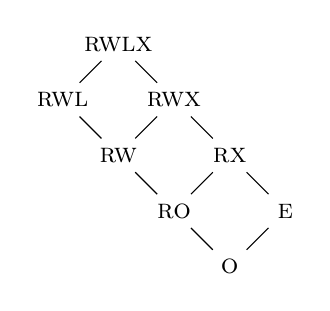
\begin{tikzpicture}[main node/.style={}]
    \node[main node] (7) {$\rwlx$};
    \node[main node] (8) [below left of=7] {$\readwritel$};
    \node[main node] (1) [below right of=7] {$\rwx$};
    \node[main node] (2) [below right of=1] {$\exec$};
    \node[main node] (3) [below right of=2] {$\entry$};
    \node[main node] (4) [below left of=1] {$\readwrite$};
    \node[main node] (5) [below right of=4] {$\readonly$};
    \node[main node] (6) [below right of=5] {$\noperm$};

    \path[every node/.style={font=\sffamily\small}]
    (7) edge (8)
    (7) edge (1)
    (8) edge (4)
    (1) edge (2)
    (2) edge (3)
    (2) edge (5)
    (3) edge (6)
    (1) edge (4)
    (4) edge (5)
    (5) edge (6);
  \end{tikzpicture}

  \caption{Permission hierarchy}
  \label{fig:perm-hier}
\end{wrapfigure}

We define the syntax of our capability machine in \figurename~\ref{fig:syntax}.
We assume an infinite set of addresses $\Addrs$ and define machine words as
either integers or capabilities of the form
$((\perm,\gl),\var{base},\var{end},\addr)$. Such a capability represents the
authority to execute permissions $\perm$ on the memory range
$[\var{base},\var{end}]$, together with a current address $\addr$ and a locality tag
$\gl$ indicating whether the capability is global or local. There is no notion
of pointers other than capabilities, so we will use the terms interchangeably.
The available permissions and their ordering are depicted in
\figurename~\ref{fig:perm-hier}: the permissions include null permission
($\noperm$), readonly ($\readonly$), read/write ($\readwrite$), read/execute
($\exec$) and read/write/execute ($\rwx$) permissions. Additionally, there are
three special permissions: read/write-local ($\readwritel$), read/write-local/execute
($\rwlx$) and enter ($\entry$), which we will explain below.

We assume a finite set of register names $\RegName$. We define register files
$\reg$ and memories $\ms$ as functions mapping register names resp. addresses to
words. The state of the entire machine is represented as a configuration that is
either a running $\Phi \in \ExecConfs$ containing a memory and a register file,
or a failed or halted state, where the latter keeps hold of the final state of
memory.
% We also define memory segments $\ms$:
% parts of memory represented as partial functions mapping addresses to words.
%\lau{we don't really make the distinction between memory and memory segments in the rest of the paper, so maybe we should leave this out?}

The machine's instruction set is rather basic. Instructions $i$ include
relatively standard jump ($\jmp{}$), conditional jump ($\jnz{}{}$) and move
($\move{}{}$, copies words between registers) instructions. Also familiar are
load and store instructions for reading from and writing to memory ($\load{}{}$
and $\store{}{}$) and arithmetic addition operators ($\lt{}{}{}$ (less than), $\plus{}{}{}$ and
$\minus{}{}{}$, operating only on numbers). There are three instructions for
modifying capabilities: $\lea{}{}$ (modifies the current address),
$\restricttwo{}{}$ (modifies the permission and local/global tag) and
$\subseg{}{}{}$ (modifies the range of a capability). Importantly, these
instructions take care that the resulting capability always carries less
authority than the original (e.g. restrict will only weaken a permission).
Finally, the instruction $\isptr{}{}$ tests whether a word is a capability or a
number and instructions $\getp{}{}$, $\getl{}{}$, $\getb{}{}$, $\gete{}{}$ and
$\geta{}{}$ provide access to a capability's permissions, local/global tag, base,
end and current address, respectively.

\begin{comment}
  \begin{figure}
    \centering
    \begin{mathpar}
      \Phi \rightarrow
      \begin{cases}
        \sem{\decode(n)}(\Phi) & \arraycolsep=0pt
        \begin{array}[t]{l}
          \text{if $\memreg(\pcreg) = \stdcap$}\\
          \;\;\text{and $\start \leq \addr \leq \addrend$ and $\memheap(\addr) = n$}\\
          \;\;\text{and $\perm \in \{ \exec,\rwx, \rwlx \}$} 
        \end{array}\\
        \failed                & \text{otherwise}
      \end{cases}
      \and \updatePcPerm{w} =
      \begin{cases}
        ((\exec,\gl),\start,\addrend,\addr) & \text{\footnotesize{if $w = ((\entry,\gl),\start,\addrend,\addr)$}}\\
        w & \text{otherwise}
      \end{cases}\\
      \and \stdUpdatePc{\Phi} =
      \begin{cases}
        \updateReg{\pcreg}{\var{newPc}} & \arraycolsep=0pt
        \begin{array}[t]{l}
          \text{if $\memreg(\pcreg) = \stdcap$}\\ 
          \;\;\text{and $\var{newPc} = ((\perm,\gl),\start,\addrend,\addr + 1)$}
        \end{array}\\
        \failed & \text{otherwise}
      \end{cases}
      \and \inferrule{ } { \sem{\fail}(\Phi) = \failed } \and
      \inferrule{ } { \sem{\halt}(\Phi) = (\halted,\memheap) } \and
      \inferrule{ } { \sem{\move{\refreg{r_1}}{r_2}}(\Phi) =
        \stdUpdatePc{}(\updateReg{r_1}{\memreg(r_2)}) } \and
      \inferrule{ \memreg(r_2) = \stdcap \\
        \perm \in \{ \rwx, \rwlx, \exec, \readwrite,
        \readwritel, \readonly \}\\
        \start \leq \addr \leq \addrend } {
        \sem{\load{\refreg{r_1}}{\refheap{r_2}}}(\Phi) =
        \updateReg{r_1}{\memheap(\addr)}} \and
      \inferrule{ \memreg(r_2) = \stdcap[\permp]\\
        \permp' = \decodePermPair{\memreg(r_2)}\\
        \permp'\sqsubseteq \permp } {
        \sem{\restricttwo{\refreg{r_1}}{r_2}}(\Phi) = \\
        \stdUpdatePc{}(\updateReg{r_1}{(\permp',\start,\addrend,\addr)})
      } \and \inferrule{ \memreg(r_2) = ((\_,\_),\_,\_,\addr) } {
        \sem{\geta{\refreg{r_1}}{\refreg{r_2}}}(\Phi) =
        \stdUpdatePc{\updateReg{r_1}{\addr}}} \and \inferrule{
        \var{newPc} = \updatePcPerm{\memreg(\lv)} } {
        \sem{\jmp{\lv}}(\Phi) = \updateReg{\pcreg}{\var{newPc}} } \and
      \inferrule{ \memreg(r_1) = \stdcap\\
        \start \leq \addr \leq \addrend\\
        \perm \in \{ \rwx, \rwlx, \readwrite, \readwritel\}\\
        \var{w} = \memreg(r_2) \\
        \var{w} = ((\_,\local),\_,\_,\_)\Rightarrow\perm \in
        \{\rwlx,\readwritel \} } {
        \sem{\store{\refheap{r_1}}{\refreg{r_2}}}(\Phi) =
        \stdUpdatePc{\updateHeap{\addr}{\var{w}}} } \and
    \end{mathpar}
    \caption{An excerpt from the operational semantics.}
    \label{fig:op-sem}
  \end{figure}
\end{comment}
\figurename~\ref{fig:op-sem} shows an excerpt of the operational semantics for a
few representative instructions. Essentially, a configuration $\Phi$ either
decodes and executes the instruction at $\memreg(\pcreg)$ if it is executable
and its address is in the valid range or otherwise fails. The table in the
figure shows for instructions $i$ the result of executing them in configuration
$\Phi$. $\fail$ and $\halt$ obviously fail and halt respectively. $\move{}{}$
simply modifies the register file as requested and updates the $\pcreg$ to the
next instruction using the meta-function $\stdUpdatePc{}$.

The $\load{}{}$ instruction loads the contents of the requested memory location
into a register, but only if the capability has appropriate authority (i.e.\
read permission and an appropriate range). $\restricttwo{}{}$ updates a
capability's permissions and global/local tag in the register file, but only if
the new permissions are weaker than the original. It also never turns local
capabilities into global ones. $\geta{}{}$ queries the current address of a
capability and stores it in a register.

The $\jmp{}$ instruction updates the program counter to a requested location,
but it is complicated by the presence of \emph{enter capabilities}, modeled
after the M-Machine's~\cite{Carter:1994:HSF:195473.195579}. Enter capabilities
cannot be used to read, write or execute and their address and range cannot be
modified. They can only be used to jump to, but when that happens, their
permission changes to $\exec$. They can be used to represent a kind of closures:
an opaque package containing a piece of code together with local encapsulated
state. Such a package can be built as an enter capability $c =
((\entry,\gl),\start,\addrend,\addr)$ where the range $[\start,\addr-1]$
contains local state (data or capabilities) and $[\addr,\addrend]$ contains
instructions. The package is opaque to an adversary holding $c$ but when $c$ is
jumped to, the instructions can start executing and have access to the local
data through the updated version of $c$ that is then in $\pcreg$\footnote{Note
that the capability in the $\pcreg$-register can be used to load from.}.  %
\lau{As we % talked about what is described here, is not how we make closures in
the TR, so % we should consider whether we should refrain from using that word
here. }

Finally, the $\store{}{}$ instruction updates the memory to the requested value
if the capability has write authority for the requested location. However, the
instruction is complicated by the presence of \emph{local capabilities}, modeled
after the ones in the CHERI processor~\cite{Watson2015Cheri}. Basically, local
capabilities are special in that they can only be kept in registers, i.e.\ they
cannot be stored to memory. This means that local capabilities can be
\emph{temporarily} given to an adversary, for the duration of an invocation: if
we take care to clear the capability from the register file after control is
passed back to us, they will not have been able to store the capability.
However, there is one exception to the rule above: local capabilities can be
stored to memory for which we have a capability with write-local authority
(i.e.\ permission $\rwl$ or $\rwlx$). This is intended to accommodate a stack,
where register contents can be stored, including local capabilities. As long as
all capabilities with write-local authority are themselves local and the stack
is cleared after control is passed back by the adversary, we will see that this
does not break the intended behavior of local capabilities.

We point out that our local capabilities capture only a part of the semantics of
local capabilities in CHERI. Specifically, in addition to the above, CHERI's
default implementation of the CCall exception handler forbids local capabilities
from being passed across module boundaries. Such a restriction fundamentally
breaks our calling convention, since we pass around local return pointers and
stack capabilities. However, CHERI's CCall is not implemented in hardware, but
in software, precisely to allow experimenting with alternative models like ours.

% Contrary to more traditional assembly languages, capability machines do not 
% allow literal addresses to appear as part of instructions. This means that we

In order to have a reasonably realistic system, we use a simple model of
linking, so programs can have access to other programs through a linking table.
We also assume malloc to be part of the trusted computing base satisfying a
certain specification. Malloc and linking tables are described further in the
next section, but we refer to the technical appendix~\cite{technical_appendix}
for full details.

\section{Stack and return pointer management using local capabilities}
\label{sec:stack-and-return-pointer} One of the contributions in this paper is a
demonstration that local capabilities on a capability machine support a calling
convention that enforces control-flow correctness in a way that is provably
watertight, potentially efficient, does not rely on a trusted central stack
manager and supports higher-order interfaces to an adversary, where an adversary
is just some unknown piece of code. In this section, we explain this
convention's high-level approach, the security measures to be taken in a number
of situations (motivating each separately with a summary table at the end).
After that, we define a number of reusable macro-instructions that can be used
to conveniently apply the proposed convention in subsequent examples.

The basic idea of our approach is simple: we stick to a single, rather standard,
C stack and register-passed stack and return pointers, much like a standard C
calling convention. However, to prevent various ways of misusing this basic
scheme, we put local capabilities to work and take a number of
not-always-obvious safety measures. In the next paragraphs, we will explain the
issues to be considered in all the relevant situations: when (1) starting our
program, (2) returning to the adversary, (3) invoking the adversary, (4)
returning from the adversary, (5) invoking an adversary callback and (6) having
a callback invoked by the adversary.

\textbf{Program start-up} We assume that the language runtime initializes the
memory as follows: a contiguous array of memory is reserved for the stack, for
which we receive a stack pointer in a special register $r_\stk$. We stress that
the stack is not built-in, but merely an abstraction we put on this piece of the
memory. The stack pointer is local and has $\rwlx$ permission. Crucially, the
stack is the only part of memory for which the runtime (including malloc,
loading, linking) will ever provide $\rwlx$ or $\rwl$ capabilities.
Additionally, our examples typically also assume some memory to store
instructions or static data. Another part of memory (called the heap) is
initially governed by malloc and at program start-up, no other code has
capabilities for this memory. Malloc hands out $\rwx$ capabilities for allocated
regions as requested (no $\rwlx$ or $\rwl$ permissions). For simplicity, we
assume that memory allocated through malloc cannot be freed.

\textbf{Returning to the adversary} Perhaps the simplest situation is returning
to the adversary after they invoked our code. In this case, we have received a
return pointer from them, and we just need to jump to it as usual. An obvious
security measure to take care of is properly clearing the non-return-value
registers before we jump (since they may contain data or capabilities that the
adversary should not get access to). Additionally, we may have used the stack
for various purposes (register spilling, storing local state when invoking other
functions etc.), so we also need to clear that data before returning to the
adversary.

However, if we are returning from a function that has itself invoked adversary
code, then clearing the used part of the stack is not enough. The \emph{unused}
part of the stack may also contain data and capabilities, left there by the
adversary, including local capabilities since the stack is write-local. As we
will see later, we rely on the fact that the adversary cannot keep hold of local
capabilities when they pass control to the trusted code and receive control
back. In this case, the adversary could use the unused part of the stack to
store local pointers and load them from there after they get control back. To
prevent this, we need to clear (i.e.\ overwrite with zeros) the entire part of
the stack that the adversary has had access to, not just the parts that we have
used ourselves. Since we may be talking about a large part of memory, this
requirement is the most problematic aspect of our calling convention for
performance, but see \sectionname~\ref{sec:discussion} for how this might be
mitigated.

\textbf{Invoking the adversary} A slightly more complex case is invoking the
adversary. As above, we clear all the non-argument registers, as well as the
part of the stack that we are not using (because, as above, it may contain local
capabilities from previously executed code that the adversary could exploit in
the same way). We leave a copy of the stack pointer in $r_\stk$, but only after
we have used the $\subseg{}{}{}$ instruction to shrink its authority to the part
that we are not using ourselves.

In one of the registers, we also provide a return pointer, which must be a local
capability. If it were global, the adversary would be able to store away the
return pointer in a global data structure (i.e.\ there exists a global capability for it), and jump to it later, in
circumstances where this should not be possible. For example, they could store
the return pointer, legally jump to it a first time, wait to be invoked again
and then jump to the old return pointer a second time, instead of the new return
pointer received for the second invocation. Similarly, they could store the
return pointer, invoke a function in our code, wait for us to invoke them again
and then jump to the old return pointer rather than the new one, received for the
second invocation.
% \lau{If we need space, then maybe one of the examples is sufficient.}
% \lau{Both of these are good to have their as the two last examples of \sectionname~\ref{sec:examples} use them.}
%
% \lau{In the examples, we refer to the local return pointer as
%   ``protected return pointer''. We should either introduce that here
%   or use a different formulation in the examples. }
% \lau{It seemed did not seem to add anything to adopt the terminlogy - we
%   often highlight that the return pointer is local which in most cases
%   is so important that we do not want to leave it out.}
By making the return pointer local, we prevent such attacks: the adversary can
only store local capabilities through write-local capabilities, which means (because
of our assumptions above): on the stack. Since the stack pointer itself is
also local, it can also only be stored on the stack. Because we clear the part
of the stack that the adversary has had access to before we pass control back,
there is no way for them to recover either of these local capabilities.

Note that storing stack pointers for use during future invocations would also be
dangerous in itself, i.e. not just because it can be used to store return
pointers. Imagine the adversary stores their stack pointer, invokes trusted code
that uses part of the stack to store private data and then invokes the adversary
again with a stack pointer restricted to exclude the part containing the private
data. If the adversary had a way of keeping hold of their old stack pointer, it
could access the private data stored there by the trusted code and break
local-state encapsulation.  
% \lau{Do we say anything about arguments to the callback? Specifically, it should not be okay to uncritically pass on argument we recieved from an adversary. Can we even to any extend allow local arguments that we pass on from an unknown source?}
% Domi: this is now discussed in the discussion section, no need to discuss it here?

\textbf{Returning from the adversary} So return pointers must be passed as local
capabilities. But what should their permissions be, what memory should they
point to and what should that memory (the activation record) contain? Let us
answer the last question first by considering what should happen when the
adversary jumps to a return pointer. In that case, the program counter should be
restored to the instruction after the jump to the adversary, so the activation
record should store this old program counter. Additionally, the stack pointer
should also be restored to its original value. Since the adversary has a more
restricted authority over the stack than the code making the call, we cannot
hope to reconstruct the original stack pointer from the stack pointer owned by the
adversary. Instead, it should be stored as part of the activation record.

\begin{figure}
  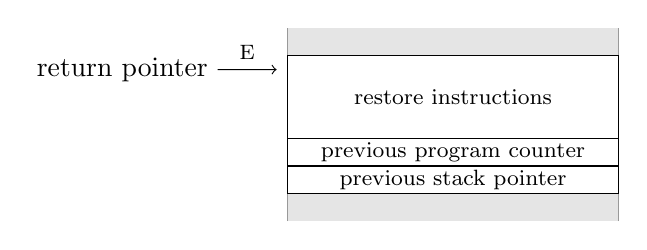
\begin{tikzpicture}[scale=.7, every node={scale=.7}]
    \draw[fill=gray!20,draw=none] (0,4) rectangle (6,3.5);
    \draw[fill=gray!20,draw=none] (0,0.5) rectangle (6,1);
    \draw[draw=gray!80] (0,0.5) -- (0,4);
    \draw[draw=gray!80] (6,0.5) -- (6,4);
    \draw (0,1) rectangle (6,1.5) node[pos=.5] {\footnotesize previous stack pointer};
    \draw (0,1.5) rectangle (6,2) node[pos=.5] {\footnotesize previous program counter};
    \draw (0,2) rectangle (6,3.5) node[pos=.5] {\footnotesize restore instructions};
    \draw (-3,3.25) node (rp) {return pointer};
    \draw[->] (rp.east) -- node[above] {$\entry$}(-.2,3.25);
  \end{tikzpicture}
  
  \caption{Structure of an activation record}
  \label{fig:activ-rec-struct}
\end{figure}

Clearly, neither of these capabilities should be accessible by the adversary. In
other words, the return pointer provided to the adversary must be a capability
that they can jump to but not read from, i.e.\ an enter capability. To make this
work, we construct the activation record as depicted in
Figure~\ref{fig:activ-rec-struct}. The $\entry$ return pointer has authority
over the entire activation record (containing the previous return and stack
pointer), and its current address points to a number of restore instructions in
the record, so that upon invocation, these instructions are executed and can
load the old stack pointer and program counter back into the register file. As
the return pointer is an enter pointer, the adversary cannot get hold of the
activation record's contents, but after invocation, its permission is updated to
$\exec$, so the contents become available to the restore instructions.

The final question that remains is: where should we store this activation
record? The attentive reader may already see that there is only one possibility:
since the activation record contains the old stack pointer, which is local, the
activation record can only be constructed in a part of memory where we have
write-local access, i.e.\ on the stack. Note that this means we will be placing
and executing instructions on the stack, i.e.\ it will not just contain code
pointers and data. This means that our calling convention should be combined
with protection against stack smashing attacks (i.e.\ buffer overflows on the
stack overwriting activation records' contents). Luckily, the capability
machine's fine-grained memory protection should make it reasonably easy for a
compiler to implement such protection, by making sure that only appropriately
bounded versions of the stack pointer are made available to source language
code.

\textbf{Invoking an adversary callback} If we have a higher-order interface to
the adversary, we may need to invoke an adversary callback. In this case, not so
much changes with respect to the situation where we invoke static adversary
code. The adversary can provide a callback as a capability for us to jump to,
either an $\entry$-capability if they want to protect themselves from us or just
an $\exec$ capability if they are not worried about that. However, there is one
scenario that we need to prevent: if they construct the callback capability to
point into the stack, it may contain local capabilities that they should not
have access to upon invocation of the callback. As before, this includes return
and stack pointers from previous stack frames that they may be
trying to illegally use inside the callback.

To prevent this, we only accept callbacks from the adversary in the form of
global capabilities, which we dynamically check before invoking them (and we
fail otherwise). This should not be an overly strict requirement: our own
callbacks do not contain local data themselves, so there should be no need for
the adversary to construct callbacks on the stack.\footnote{Note that it does
  prevent a legitimate but non-essential scenario where the adversary wants to
  give us temporary access to a callback not allocated on the stack.}

\textbf{Having a callback invoked by the adversary} The above leaves us with
perhaps the hardest scenario: how to provide a callback to the adversary. The
basic idea is that we allocate a block of memory using malloc that we fill with
the capabilities and data that the callback needs, as well as some
prelude instructions that load the data into registers and jumps to the right
code. Note that this implies that no local capabilities can be stored as part of
a closure. We can then provide the adversary with an enter-capability covering
the allocated block and pointing to the contained prelude instructions. However,
the question that remains in this setup is: from where do we get a stack pointer when
the callback is invoked?

Our answer is that the adversary should provide it to us, just as we provide
them with a stack pointer when we invoke their code. However, it is important
that we do not just accept any capability as a stack pointer but check that it
is safe to use. Specifically, we check that it is indeed an $\rwlx$ capability. Without
this check, an adversary could potentially get control over our local stack
frame during a subsequent callback by passing us a local $\rwx$ capability to a global data
structure instead of a proper stack pointer
and a global callback for our callback to invoke. If our local state contains no
local capabilities, then, following our calling convention, the callback would
not fail and the adversary could use a stored capability for the global data
structure to access our local state. To prevent this from happening, we need to
make sure the stack capability carries $\rwlx$ authority, since the system wide assumption then
tells us that the adversary cannot have global capabilities to our local stack.

\textbf{Calling convention} With the security measures introduced and motivated,
let us summarize our proposed calling convention: \textit{At program start-up} A
local $\rwlx$ stack pointer resides in register $r_\stk$. No global write-local
capabilities. \textit{Before returning to the adversary} Clear non-return-value
registers. Clear the part of the stack we had access to (not just the part we
used). \textit{Before invoking the adversary} Push activation record to the
stack. Create return pointer as local $\entry$-capability to the instructions in
the record.  Restrict the stack capability to the unused part and clear
it. Clear non-argument registers. \textit{Before invoking an adversary callback}
Make sure callback is global. \textit{When invoked by an adversary} Make sure
received stack pointer has permission $\rwlx$.

\textbf{Reusable macro instructions} We define a number of reusable
macros capturing the calling convention and other conveniences. All
macros that use the stack assume a stack pointer in register
$r_\stk$. The macro \texttt{\footnotesize{fetch $r$ $\var{name}$}} fetches the
capability related to $\var{name}$ from the linking table and stores
it in register $r$.  The macros \texttt{\footnotesize{push $r$}} and
\texttt{\footnotesize{pop $r$}} work as one would
expect. The macro \texttt{\footnotesize{prepstk $r$}} is used when a callback is
invoked by the adversary and prepares the received stack pointer by
checking that it has permission $\rwlx$.  The macro \texttt{\footnotesize{scall
    $r$($\overline{r_{\var{args}}}$,$\overline{r_{\var{priv}}}$)}}
jumps to the capability in register $r$ in the manner described
above. That is, it pushes local state (the contents of registers
$\overline{r_{\var{priv}}}$) and the activation record (return code,
return pointer, stack pointer) to the stack, creates an $\entry$
return pointer, restricts the stack pointer, clears the unused part of
the stack, clears the necessary registers and jumps to $r$.  Upon
return, the private state is restored. The macro \texttt{\footnotesize{mclear
    $r$}} clears all the memory the capability in register $r$ has
authority over.  The macro \texttt{\footnotesize{rclear $\var{regSet}$}} clears
all the registers in $\var{regSet}$. The macro \texttt{\footnotesize{reqglob
    $r$}} checks whether the word in register $r$ is a global
capability. The macro \texttt{\footnotesize{crtcls $\overline{(x_i,r_i)}$ $r$}}
allocates a closure where $r$ points to the closure's code and a new
environment is allocated (using malloc) where the contents of
$\overline{r_i}$ is stored. In the code referred to by $r$, an
implicit fetch happens when an instruction refers to $x_i$.

The technical appendix~\cite{technical_appendix} contains detailed descriptions
of all the macros.

\section{Logical relation}
\label{sec:logical-relation}

In this section, we formalize the guarantees provided by the
capability machine, including the specific guarantees for local
capabilities, by means of a step-indexed Kripke logical relation 
with recursively defined worlds. 
We use the logical relation in the following section to show
local-state encapsulation and control-flow integrity properties for
challenging example programs.

% Our logical relation will prescribe which values are capability safe given a
% world $W$ containing a set of memory invariants. For expressiveness,
% we use invariants which can evolve over time (sometimes also referred
% to as \emph{protocols}). We thus start by describing the worlds we
% will use.


% Now that we have defined our calling convention, how can we be sure that it
% works? More concretely, suppose that we have a program that uses the convention
% in its interaction with untrusted adversary code. Can we formally prove the
% program's correctness if it relies on well-bracketed control flow and private
% state encapsulation for the interaction with the adversary? Clearly, such a
% proof should depend on a formal expression of the guarantees provided by the
% capability machine, including the specific guarantees for local capabilities.

% In this section, we construct such a formalization. We make use of some
% well-studied and powerful (but non-trivial) machinery from the literature.
% Specifically, we employ a unary step-indexed Kripke logical relation with
% recursive worlds, and some additional special characteristics of our own.
% Step-indexing, Kripke logical relations and recursive worlds are techniques that
% may be familiar from lambda calculus settings, but it may not be clear to the
% reader how they apply in this more low-level assembly language. Therefore, we do
% not immediately dive into the details, but we first try to provide some informal
% intuition about how all of this machinery comes into play in our setting, in the
% next section.

% Note: even though the calling convention is the main application in this paper,
% the logical relation we construct is very general and should be regarded as an
% independent contribution.

% \subsection{Formalizing the guarantees of the capability machine}
% \label{sec:formalizing-guarantees}
% What differentiates a capability machine from a more standard assembly language
% is that we can bound the authority of an executing block of code, based solely
% on the capabilities it has access to. Specifically, it does not matter which
% instructions are actually executed, i.e., the bound also applies to untrusted
% adversary code that has not been inspected or modified in any way.

% \paragraph{Worlds}
% But what does a ``bound on the authority'' of an executing block of code mean?
% In our setting, there are no externally observable side-effects and the only
% primitive authority that code may hold is authority over memory. As such, the
% authority bounds we consider are related to memory, but in a form that is more
% fine-grained than standard read/write authority: a piece of code's authority can be bounded
% by arbitrary memory invariants that it is required to respect. Specifically, we
% will define worlds $W \in \Worlds$, which describe a set of memory invariants, and
% our results will express authority bounds on code as \emph{safety with respect to such
% a world,} i.e., the fact that the code respects the invariants registered in
% the world.

% \paragraph{Safe values}
% So, let's say that we have a world $W$ expressing that the memory must contain
% value $42$ at address $0$, may contain arbitrary values at
% addresses $50$-$60$, a $\readwrite$ capability for address $0$ at address $73$, and
% an integer at address $100$ that may only increase over time\footnote{Indeed, we
%   will allow a notion of \emph{evolvable} invariants, aka \emph{protocols}, that can
%   express such a temporal property.}. Our main theorem will state that if the
% current register file only contains safe words (numbers or capabilities which
% preserve the invariants in $W$ under any interaction), then an execution will
% necessarily also preserve the memory invariants (irrespective of the instructions being
% executed).

% To make this more precise, we need to define the set $\stdvr(W) \in
% \powerset{\Words}$ of words that are safe w.r.t.\ $W$. Essentially, the set
% should only include words that preserve $W$'s invariants under any interaction,
% but should otherwise be as liberal as possible. Numbers are clearly always safe,
% as they cannot be used to break invariants. Whether a capability is safe depends
% on the authority that it carries. In the above-described world, a read capability
% for address $0$ is safe, as it can only be used to read the value $42$, which is
% itself safe. However, a write capability for address $0$ is not safe: it can be
% used to overwrite the memory at that address with a value other than $42$,
% breaking the invariant for that address.

% \paragraph{Step-indexing}
% More generally, we want to define that a read capability for memory range
% $[b,e]$ is safe, if the world guarantees that the words at those addresses are
% themselves safe. However, this definition is cyclic: what if the world
% guarantees that the memory at address $a$ will contain a read capability for
% address $a$? The definition then just says that a read capability for address
% $a$ is safe if and only if the same read capability for address $a$ is safe. This form of
% cyclic reasoning is related to similar challenges in languages with recursive
% types or higher-order ML-style references, and a standard solution is
% to use step-indexing \cite{Appel:2001:IMR:504709.504712}: essentially, the cycle is broken by defining safety up to a
% certain number of interaction steps. All words will be considered
% safe up to $0$ steps (since if there is no interaction, nothing unsafe
% can happen), and, for example, a read capability will be safe up to $n$
% steps if the world guarantees that the words at the corresponding addresses are
% safe up to $n - 1$ steps. We can then prove that the above read capability for
% address $a$ is safe up to any number of steps.

% \paragraph{Future worlds}
% So worlds are defined as a set of invariants on the memory, but what if we
% allocate fresh memory through malloc? We may want to establish new invariants
% for this freshly allocated memory and be sure that the adversary will also
% respect those (if we don't provide them with capabilities through which the new
% invariants can be broken). To accommodate this, we allow worlds to evolve, for
% example by adding additional invariants for freshly allocated memory. Formally,
% we define valid ways for a world $W$ to evolve into a new world $W'$ through a
% future-world relation $W' \future W$ and we ensure that the set of safe words in
% world $W$ must remain safe in any future world $W'$. Defining safety w.r.t.\ a
% notion of evolvable worlds makes our logical relation into a \emph{Kripke}
% logical relation \cite{pitts_operational_1998}.

% \paragraph{Invariants and Recursive Worlds}
% So worlds group a set of memory invariants, but how are they actually
% defined formally? We represent each invariant by a region
% $r \in \Regions$. We will see later that regions contain state
% machines to support a notion of evolvable invariants, but in every
% state, they also contain a predicate $H$ that defines which memory
% segments are acceptable in the current state of the invariant.
% Unfortunately, it is not enough to just take
% $H \in \powerset{\MemSegments}$, because sometimes the invariant may
% itself be world-dependent. For example, we may want to express
% invariants like ``the memory at address $50$ contains a value that is
% safe in the current world''. As explained, worlds may evolve, and the
% set of safe values may grow in future worlds, and therefore we need to
% index $H$ over worlds, i.e., take
% $H \in \Worlds \rightarrow \powerset{\MemSegments}$. We then end up
% with worlds containing regions with world-indexed predicates,
% i.e., the set of worlds must be recursively defined. We will see how such a recursive
% definition can be accommodated using techniques from the
% literature (essentially an advanced application of step-indexing).

% \paragraph{Local capabilities}
% A final thing we provide informal intuition for is how our results take into account local
% capabilities and their special treatment by the hardware. Normally, when we
% invoke an untrusted piece of code and provide it with certain global
% capabilities, it may have stored those capabilities in memory and we will only
% be able to reinvoke the code if we can guarantee that those values are still
% valid. Formally, worlds represent the invariants that global capabilities'
% safety relies on and the reinvocation is only safe in future worlds, where the
% invariants are respected.

% However, if we provide the adversary with local capabilities in that first
% invocation, then the situation is a bit different. The adversary has no way to
% store these local capabilities, so if we make sure that there are also no old
% local capabilities in the register file for the second invocation (including the
% capability being invoked), then the adversary cannot use them any more.%
% \footnote{We are ignoring write-local capabilities in this discussion. If the
%   adversary does have access to write-local capabilities in the first and second
%   invocation, then the memory they address must entirely be cleared before the
%   second invocation in order for the reinvocation to remain safe.} Therefore, we
% can allow the second invocation to happen in \emph{private} future worlds ($W'
% \futurestr W$), in which safe global capabilities remain safe, but local ones
% don't. This private future world relation is more liberal than the standard,
% public one ($W' \futurewk W$, in which \emph{all} safe capabilities remain
% safe). Concretely, worlds may contain \emph{temporary} regions, representing
% invariants that only local capabilities may rely on for their safety, and which
% may be revoked (disabled) in private future worlds.

% Interestingly, this idea is a variant of a notion of public/private future
% worlds that has been previously used in the literature (see
% \sectionname~\ref{sec:discussion}). However, temporary regions are new in our setting
% and there is an interesting interplay with the recursiveness of the worlds: for
% a temporary region, the predicate $H \in \Worlds \rightarrow
% \powerset{\MemSegments}$ (which defines the safe memory segments in the
% current world) is only required to be monotone w.r.t.\ public
% future worlds (i.e.\ safe memory segments remain safe in public future worlds),
% but for permanent regions, it must be monotone w.r.t.\ private future worlds.
% As a consequence, the memory for a permanent region may not contain local
% capabilities (as their safety would be broken in private future worlds), which
% in turn implies that only local capabilities may have write-local permission (a
% general sanity requirement when using local capabilities\footnote{In fact, local
%   capabilities become useless as soon as the adversary has access to a single
%   global, write-local capability.})\footnote{For explanation purposes, this
%   discussion ignores certain ways to allow for local capabilities in a permanent
%   region, for example, by not requiring that they are valid or requiring that
%   they are local versions of valid global capabilities.}.

\subsection{Worlds}
\begin{figure}
  \centering
  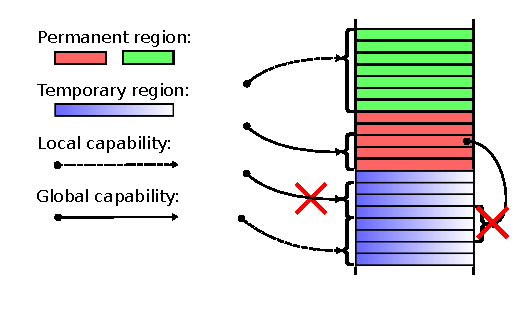
\includegraphics{w11}

  \caption{The relation between local/global capabilities and temporary/permanent
    regions. The colored fields are regions governing parts of memory. Global capabilities cannot depend on temporary
    regions.}
  \label{fig:cap-world}
\end{figure}
% \dominique{Perhaps we could first try to convey the intuition of a permanent
%   world with a temporary overlay, with global capabilities ignoring the overlay.
%   Perhaps we could add a depiction of the world to Figure 5?}
%\todo[inline]{Find a good place to describe monotonicity of
%interpretation function.}
% \lau{this may not be an important enough point to include it.}

%As describe above, worlds are a collection of invariants. Formally, 

A world is a
finite map from region names, modeled as natural numbers, to regions that each
correspond to an invariant of part of the memory.  We have three types of
regions: \emph{permanent}, \emph{temporary}, and \emph{revoked}.
%$\perma$, $\temp$, and $\revoked$. The
%$\perma$ and $\temp$ 
Each permanent and temporary region contains a state transition system, with
public and private transitions, to describe how the invariants are allowed to
change over time. In other words, they are protocols for the region's
memory. These are similar to what has been used in logical relations for
high-level
languages~\cite{Ahmed:popl09,Dreyer:jfp12,Devriese:2016ObjCap}. Protocols
imposed by permanent regions stay in place indefinitely. Any capability, local
or global, can depend on these protocols. Protocols imposed by temporary regions
can be revoked in private future worlds. Doing this may break the safety of
local capabilities but not global ones. This means that local capabilities
can safely depend on the protocols imposed by temporary regions, but global
capabilities cannot, since a global capability may outlive a temporary region
that is revoked. This is illustrated in \figurename~\ref{fig:cap-world}.

For technical reasons, we do not actually remove a revoked temporary region from
the world, but we turn it into a special revoked region that exists for this purpose.
Such a revoked region contains no state transition system and puts no
requirements on the memory. It simply serves as a mask for a revoked temporary
region. Masking a region like this goes back to earlier work of
\cite{Ahmed2004semantics} and was also used by
\cite{Thamsborg:2011:KLR:2034773.2034831}.

% Recursive worlds intuition
% The worlds end up being defined recursively: The memory can contain
% capabilities,
% which grant authority over parts of memory. A world
% models memory, so it also needs to be able to model capabilities in
% memory and the protocols on them. Whether a capability satisfies the
% protocol of a region may depend on what it grants authority over in
% memory which is described by the world.

%\dominique{``end up being defined recursively'' does not sound very insightful}
% A region defines what its part of memory can legally look like. However,
% validity of the memory's contents may itself depend on the state of other parts
% of memory. To accommodate this, worlds need to be defined recursively: Worlds
% describe memory, which can contain capabilities, whose safety is
% world-dependent. 
%As described in \sectionname~\ref{sec:formalizing-guarantees}, regions define sets of

Regions are used to define safe memory segments, but this set may itself be world-dependent. In other
words, our worlds are defined recursively. Recursive worlds are common
in Kripke models and the following lemma uses the method of
\cite{Birkedal:2011:SKM:1926385.1926401,Birkedal:tutorial-notes} for
constructing them. The formulation of the lemma is technical, so we recommend
that non-expert readers ignore the technicalities and accept that there exists a
set of worlds $\Wor$ and two relations $\futurestr$ and $\futurewk$ satisfying
the (recursive) equations in the theorem (where the $\blater$ operator can be
safely ignored).
% Short technical explanation
% The recursiveness of the worlds gives rise to a recurisve domain
% equation. Theorem~\ref{thm:world-existence} gives the solution to this
% recursive domain equation.
% \dominique{it is not explained what cofes are?}
% \lau{I added what cofe means but no formal definition (I think this goes under the category technicalities)}
\begin{theorem}\label{thm:world-existence}
  There exists a \cofe{} (complete ordered family of equivalences) $\Wor$ and preorders $\futurestr$ and
  $\futurewk$ such that $(\Wor,\futurestr)$ and $(\Wor,\futurewk)$ are
  preordered \cofes{}, and there exists an isomorphism $\xi$ such that
  \begin{align*}
      \xi \; : \; & \Wor \cong \blater (\nats \finparfun \Regions)\\
      \Regions  = & \; \{\revoked\} \uplus \\
               & \; \{\temp\} \times \States \times \Rels \times (\States \fun (\Wor \monwknefun \UPred{\HeapSegments}))\uplus \\
               & \; \{\perma\} \times \States \times \Rels \times (\States \fun (\Wor \monstrnefun \UPred{\HeapSegments}))
    \end{align*}
  and for $W, W' \in \Wor\ldotp \quad  
  \begin{aligned}
    W' \futurestr W & \Leftrightarrow \xi(W') \futurestr \xi(W)   \\
    W' \futurewk W & \Leftrightarrow \xi(W') \futurewk \xi(W)
  \end{aligned}$
\end{theorem}
In the above theorem, $\States \times \Rels$ corresponds to the aforementioned
state transition system where $\Rels$ contains pairs of relations corresponding
to the public and private transitions, and $\States$ is an unspecified set that
we assume to contain at least the states we use in this paper. The last part of
the temporary and permanent regions is a state interpretation function that
determines what memory segments the region permits in each state of the state
transition system.  The different monotonicity requirements in the two
interpretation functions reflects how permanent regions rely only on permanent
protocols whereas temporary regions can rely on both temporary and permanent
protocols.  $\UPred{\HeapSegments}$ is the set of step-indexed, downwards closed
predicates on memory segments:
$\UPred{\HeapSegments} = \{ A \subseteq  \nats \times
\HeapSegments \mid 
\forall (n, ms) \in A. \forall m
\leq n. (m, ms) \in A\}$. 
\

With the recursive domain equation solved, we could take $\Wor$ as our notion of
worlds, but it is technically more convenient to work with the following
definition instead:
\[
  \Worlds = \nats \finparfun \Regions
\]

\subsubsection{Future worlds}
\label{subsec:future-worlds} 
The future world relations model how memory may evolve over time. 
The \emph{public future world} $W' \futurewk W$ requires that $\dom(W') \supseteq
\dom(W)$ and $\forall r \in \dom(W) \ldotp W'(r) \futurewk W(r)$. That is, in a
public future world, new regions may have been allocated, and existing regions
may have evolved according to the public future region relation (defined below).
The \emph{private future world} relation $W' \futurestr W$ is defined similarly,
using a private future region relation. The \emph{public future} region relation is the simplest. It satisfies
% \dominique{is defined by?} 
% \lau{As I have understood it, the relation from the theorem defines the future world relations and indirectly the future region relations. It can be shown that these will have the properties mentioned below}
the following properties:
\begin{mathpar}
  \inferrule{ (s,s') \in \phi_\pub }
  {  (v,s',\phi_\pub,\phi,H) \futurewk (v,s,\phi_\pub,\phi,H) }
  \and
  \inferrule{ (\temp,s,\phi_\pub,\phi,H) \in \Regions }
  { (\temp,s,\phi_\pub,\phi,H) \futurewk \revoked }
  \and
  \inferrule{ }
  { \revoked \futurewk \revoked }
\end{mathpar}
Both temporary and permanent regions are only allowed to transition according to
the public part of their transition system. Additionally, revoked regions must
either remain revoked or be replaced by a temporary region. This means that the
public future world relations allows us to reinstate a region that has been revoked
earlier. The \emph{private future region} relation satisfies:
\begin{mathpar}
  \inferrule{ (s,s') \in \phi} 
  {  (v,s',\phi_\pub,\phi,H) \futurestr (v,s,\phi_\pub,\phi,H) }
  \and
  \inferrule{ r \in \Regions }
  { r \futurestr (\temp,s,\phi_\pub,\phi,H) }
  \and
  \inferrule{ r \in \Regions }
  { r \futurestr \revoked }
\end{mathpar}
Here, revocation of temporary regions is allowed. In fact, temporary regions can
be replaced by an arbitrary other region, not just the special $\revoked$.
Conversely, $\revoked$ regions may also be replaced by any other region. On
the other hand, permanent regions cannot be masked away. They are only allowed
to transition according to the private part of the transition system.

Notice that the public future region relation is a subset of the private future
region relation.
%domi: the below seems hard to understand at this moment.
% The public future region relation only allows revoked regions
% to be reused as temporary region. This means that it is always possible to turn
% it back into a revoked region in a private future region. This requirement turns
% out to be important in order to be able to restore the invariants of a caller.

%%%%%%%%

% In order to model changes to memory over time, we use the future world
% relations. The future world relations model how more memory may be
% allocated but also how memory may change. How memory is allowed to
% change over time depends on the region that governs it and the future
% world relation used. The most interesting part about the future worlds
% is how it affects the regions, so we first look at the properties of
% the \emph{public future region} relation and the \emph{private future
%   region} relation. We then use these relations to describe the future
% world relations.

% {\bf Private future regions}
% In the private future region relation, we allow revocation of $\temp$
% regions. The regions cannot be revoked by removing them from the
% world, because we need the future world relations to be
% monotone. This is why we have the $\revoked$ region, so we have
% a region that can serve as a mask. We can, however, let any region
% serve as a mask, so in the private future region relation, we allow a
% $\temp$ region to become any valid region. As the $\revoked$ region
% serves as a mask, we let any valid region take its place in the
% private future region relation.

% If a $\temp$ region is not masked by a region, then it behaved like a
% $\perm$ region. The $\perma$ regions stay the same type and they are
% allowed to take a transition in the private part of the transition
% system. Which can be thought of as the memory changes according to
% some protocol.

% The properties of the \emph{private future region} relation are:
% \begin{mathpar}
%   \inferrule{  (s,s') \in \phi \\
%     (v,\phi_\pub,\phi,H) = (v',\phi_\pub',\phi',H')}
%   {  (v',s',\phi_\pub',\phi',H') \futurestr (v,s,\phi_\pub,\phi,H) }
%   \and
%   \inferrule{ r \in \Regions }
%   { r \futurestr (\temp,s,\phi_\pub,\phi,H) }
%   \and
%   \inferrule{ r \in \Regions }
%   { r \futurestr \revoked }
% \end{mathpar}

% {\bf Public future regions}
% In the public future regions we do not permit revocation of $\temp$
% regions. In this relation, the $\temp$ and $\perma$ regions must stay
% the same type and they are allowed to take a transition in the public
% part of the transition system.

% The $\revoked$ regions serve as masking regions, but are not as
% liberal as in the private future region relation when it comes to
% letting other regions replace them as masks. In the public future
% region relation, we only allow $\revoked$ and $\temp$ regions to take
% on the job as masking region. We have this limitation, because we
% want the private future region relation to be able to reuse any region
% it has revoked.

% The \emph{public future} region relations satisfies the following properties:
% \begin{mathpar}
%   \inferrule{  (s,s') \in \phi_\pub \\
%     (v,\phi_\pub,\phi,H) = (v',\phi_\pub',\phi',H')}
%   {  (v',s',\phi_\pub',\phi',H') \futurewk (v,s,\phi_\pub,\phi,H) }
%   \and
%   \inferrule{ (\temp,s,\phi_\pub,\phi,H) \in \Regions }
%   { (\temp,s,\phi_\pub,\phi,H) \futurewk \revoked }
%   \and
%   \inferrule{ }
%   { \revoked \futurewk \revoked }
% \end{mathpar}

% Notice that the public future region relation is a subset of the
% private future region relation, so anything you are allowed to do in
% the public future region relation, the private future region relation
% can do the same.


% % The future world relation are really the ones from thm, the above
% % are properties of them.
% {\bf Future world relations}
% There are two future world relations a \emph{public future world}
% relation and a \emph{private future world} relation. In both future
% world relations, we have extension ordering, so a future world $W'$ of
% $W$ has at least the same regions as $W$, but $W'$ may have new regions
% imposing new protocols on parts of the memory. The two future world
% relations differ in the way existing regions are allowed to
% evolve. The public future world relation uses the public future region
% relation and the private future world relation uses the private future
% region relation:
% \begin{mathpar}
%   \inferrule{ \dom(W') \supseteq \dom(W)\\ 
%     \forall r \in \dom(W) \ldotp W'(r) \futurewk W(r) }
%   { W' \futurewk W }
%   \and
%   \inferrule{ \dom(W') \supseteq \dom(W)\\ 
%     \forall r \in \dom(W) \ldotp W'(r) \futurestr W(r) }
%   { W' \futurestr W }
% \end{mathpar}

% % Relate to STSs for high-level languages. Have the public-private
% % transitions, but they are also used for more than this
% \todo[inline]{Relate to STSs for high-level languages?}

\subsubsection{World satisfaction}
A memory satisfies a world, written $\memSat{\ms}{W}$, if it can be partitioned
into disjoint parts such that each part is accepted by an active (permanent or
temporary) region.  Revoked regions are not taken into account as their memory protocols are no longer in effect.
\begin{align*}
  &\memSat{\ms}{W}
    \text{ iff }\quad \left\{\begin{aligned}
        &\exists P : \activeReg{W} \rightarrow \HeapSegments \ldotp \hs = \biguplus_{r\in\activeReg{W}}P(r) \text{ and } \\[-.35cm]
        &\quad \forall r \in \activeReg{W} \ldotp\\
        &\quad \quad \exists H,s \ldotp W(r) = (\_,s,\_,\_,H) \text{ and } \npair[n]{P(r)} \in H(s)(\xi^{-1}(W))\\
      \end{aligned}\right.
\end{align*}
% LB: omitted the following for brevity:
% Note that it is possible to state nonsensical worlds with conflicting
% requirements for the same part of memory. There would, however, be no
% memory that would satisfy such a world which for all intents and purposes would
% make it discounted by the logical relation.

\subsection{Logical relation}
\afterpage{
\begin{figure}[htbp]
  \centering
%  \begin{withmathindent}{0cm}
    \begin{align*}
      & \observations \; : \;  \Worlds \nefun \UPred{\Regs \times \HeapSegments} \\
      & \observations (W) \defeq 
        \;\left\{ \npair{(\reg,\ms)} \; \middle| \;
        \begin{aligned}
          & \forall \ms_f, \heap', i \leq n \ldotp  (\reg,\ms \uplus \ms_f) \step[i] (\halted,\heap') \Rightarrow \\
          & \;\; %\Rightarrow
            \exists W' \futurestr W, \ms_r, \ms' \ldotp \\
          & \;\;\;\; \heap' = \ms' \uplus \ms_r \uplus \ms_f \text{ and } \heapSat[\hs']{n-i}{W'}
        \end{aligned}\right\}\\
      & \stdrr \; : \; \Worlds \monwknefun \UPred{\Regs} \\
      & \stdrr(W) \defeq \left\{ \npair{\reg} \; \middle| \;
          \forall r \in \RegName \setminus \{\pcreg\} \ldotp \npair{\reg(r)}
          \in \stdvr(W) \right\} \\
      & \\[-.2cm]
      & \stder \; : \; \Worlds \nefun \UPred{\Words} \\
      & \stder(W) \defeq \left\{ \npair{\pc} \; \middle| \;
        \begin{multlined}
          \forall n' \leq n, \npair[n']{\reg} \in \stdrr(W), \heapSat[\hs]{n'}{W} \ldotp \\
          \npair[n']{(\reg\update{\pcreg}{\pc},\hs)} \in \observations(W)
        \end{multlined} \right\} \\
      & \\[-0.2cm]
      &\stdvr \; : \; \Worlds \monwknefun \UPred{\Words} \\
      &\stdvr(W)\defeq 
        \begin{aligned}[t] & \{ \npair{i} \mid i \in \ints \} \union \{ \npair{\stdcap[(\noperm,\gl)] } \}
        \union \\
        % & \left\{
        %     \npair{\stdcap[(\readonly,\gl)] } \mid \npair{(\start,\addrend)} \in \readCond{}(\gl)(W)
        %   \right\}
        % \union \\
        & \left\{
            \npair{\stdcap[(\readwrite,\gl)] } \; \middle| \;
            \begin{array}{l}
              \npair{(\start,\addrend)} \in \readCond{}(\gl)(W) \text{ and } \\
              \npair{(\start,\addrend)} \in \writeCond{}(\iota^\nwl,\gl)(W)
            \end{array}
          \right\} \union \\
        % & \left\{
        %     \npair{\stdcap[(\readwritel,\gl)] } \;\middle| \;
        %     \begin{array}{l}
        %      \npair{(\start,\addrend)} \in \readCond{}(\gl)(W) \text{ and } \\
        %      \npair{(\start,\addrend)} \in \writeCond{}(\iota^\pwl,\gl)(W)
        %     \end{array}
        %    \right\}
        % \union \\
        % & \left\{
        %   \npair{\stdcap[(\exec,\gl)]} \; \middle| \;
        %   \begin{array}{l}
        %      \npair{(\start,\addrend)} \in \readCond{}(\gl)(W) \text{ and } \\
        %      \npair{(\{\exec\},\start,\addrend)} \in \execCond{}(\gl)(W)
        %   \end{array}
        %    \right\}
        % \union \\
        & \left\{
            \npair{\stdcap[(\entry,\gl)]} \; \middle| \;
            \npair{(\start,\addrend,\addr)} \in \entryCond{}(\gl)(W)
          \right\}
        \union \\ 
        % & \left\{
        %   \npair{\stdcap[(\rwx,\gl)]}\; \middle| \; 
        %   \begin{array}{l}
        %     \npair{(\start,\addrend)} \in \readCond{}(\gl)(W) \text{ and } \\
        %     \npair{(\start,\addrend)} \in \writeCond{}(\iota^\nwl,\gl)(W) \text{ and }\\
        %     \npair{(\{\rwx,\exec\},\start,\addrend)} \in \execCond{}(\gl)(W)
        %   \end{array}
        %   \right\}
        % \union \\
        & \left\{
            \npair{\stdcap[(\rwlx,\gl)]} \; \middle| \;
            \begin{array}{l}
             \npair{(\start,\addrend)} \in \readCond{}(\gl)(W) \text{ and } \\
             \npair{(\start,\addrend)} \in \writeCond{}(\iota^\pwl,\gl)(W) \text{ and }\\
             \npair{(\{\rwlx,\rwx,\exec\},\start,\addrend)} \in \execCond{}(\gl)(W)
            \end{array}
          \right\} \\
          \union
        & \dots \small{\text{\itshape and so on for permissions $\readonly$, $\readwritel$, $\exec$, and $\rwx$.}}
      \end{aligned}
    \end{align*}
%  \end{withmathindent}
  \caption{Logical relation}
  \label{fig:logrel}            
\end{figure}


% \begin{figure}[htbp]
%   \centering
%   \begin{align*}
%   &\iota_{\start,\addrend}^\pwl : \Regions\\
%   &\iota_{\start,\addrend}^\pwl \defeq (\temp,1,=,=,H^\pwl_{\start,\addrend}) \\
%   \\
%   &H^\pwl : \Addrs^2 \fun \States \fun (\Wor \monwknefun \UPred{\HeapSegments})\\
%   &H^\pwl_{\start,\addrend}\; s \; \hat{W} \defeq  \quad\left\{\npair{\hs} \; \middle| \;
%     \begin{aligned}
%       & n = 0 \text{\footnotesize{ or }} (\dom(\hs) = [\start,\addrend] \text{\footnotesize{ and }} \\
%       &\forall \addr \in [\start,\addrend] \ldotp\\
%       & \;\; \npair[n-1]{\hs(\addr)} \in \stdvr(\xi(\hat{W})))
%     \end{aligned}
%         \right\}\\
%   &\iota_{\start,\addrend}^{\nwl} : \Regions \\
%   &\iota_{\start,\addrend}^{\nwl} \defeq (\temp,1,=,=,H^\nwl_{start,\addrend}) \\
%   \\
%   &H^\nwl : \Addrs^2 \fun \States \fun (\Wor \monstrnefun \UPred{\HeapSegments})\\
%   &H^\nwl_{\start,\addrend} \; s \;\hat{W} \defeq \quad\left\{\npair{\hs} \; \middle| \;
%     \begin{aligned}
%       &n = 0 \text{\footnotesize{ or }} (\dom(\hs) = [\start,\addrend] \text{\footnotesize{ and }}\\
%       &\forall \addr \in [\start,\addrend] \ldotp \\
%       & \;\; {\footnotesize\nonlocal{\ms(\addr)}} \text{\footnotesize{ and }}\\
%       & \;\; \npair[n-1]{\hs(\addr)} \in \stdvr(\xi(\hat{W})))
%      \end{aligned}
%      \right\}
% \end{align*}
% \caption{Standard regions}
% \label{fig:standard-regions}
% \end{figure}


\begin{figure}[htbp]
  \centering
  \begin{align*}
   \readCond{}(\gl)(W) &=  \left\{ \npair{(\start,\addrend)} \; \middle| \;
    \begin{array}{l}
       \exists r \in \var{localityReg}(g,W) \ldotp \\
\quad   \exists [\start',\addrend'] \supseteq [\start,\addrend] \ldotp W(r)\nsubsim[n] \iota_{\start',\addrend'}^\pwl 
    \end{array}
    \right\}\\
   \writeCond{}(\iota,\gl)(W) &=  \left\{
    \npair{(\start,\addrend)}
    \; \middle| \;
    \begin{aligned}
      & \exists r \in \var{localityReg}(g,W) \ldotp \\
      & W(r) \text{ is address-stratified and} \\[-0.2cm]
      & \;\; \exists [\start',\addrend'] \supseteq [\start,\addrend] \ldotp W(r)\nsupsim[n-1] \iota_{\start',\addrend'}
    \end{aligned} \right\}\\
   \execCond{}(\gl)(W) &= 
    \left\{
      \npairP{(\var{P}, \start,\addrend)}
     \; \middle| \;
    \begin{aligned}
      & \forall n' < n, W' \future W, a \in [\start,\addrend], \perm \in \var{P} \ldotp \\
      & \;\;\;\; \npair[n']{((\perm,\gl),\start,\addrend,\addr)} \in \stder(W')\\
    \end{aligned} \right\} \\
   \entryCond{}(\gl)(W) &= 
    \left\{ \npair{(\start,\addrend,\addr)} \; \middle| \;
    \begin{array}{l}
      \forall n' < n \ldotp \forall W' \future W \ldotp\\
      \quad \npair[n']{((\exec,\gl),\start,\addrend,\addr)} \in \stder(W')
    \end{array}
    \right\} \\
   \text{where } \gl = \local \Rightarrow \future = \futurewk \text{ and } \gl = \glob \Rightarrow \future = \futurestr \span
  \end{align*}
\caption{Permission-based conditions}
\label{fig:perm-conds}
\end{figure}
}
%subsection introduction
% \dominique{I would try to motivate the LR defs by saying that the LR is
%   constructed to express the FTLR and the FTLR says that if a piece of code only
%   has access to values respecting the invariants in a world, then it will
%   respect them itself too.} 
The logical relation defines semantically when values, program
counters, and configurations are capability safe. The definition is
found in \figurename{}s~\ref{fig:logrel} and~\ref{fig:perm-conds} and
we provide some explanations in the following paragraphs. For space
reasons, we omit some definitions and explain them only verbally, but
precise definitions can be found in the technical
appendix~\cite{technical_appendix}.

First, the \emph{observation relation} $\observations$ defines what
configurations we consider safe. A configuration is safe
with respect to a world, when the execution of said configuration does not break
the memory protocols of the world. Roughly speaking, this means that when the
execution of a configuration halts, then there is a private future world that
the resulting memory satisfies. Notice that failing is considered safe behavior.
In fact, the machine often resorts to failing when an unauthorized access is
attempted, like loading from a capability without read permission. This is
similar to \cite{Devriese:2016ObjCap}'s logical relation for an untyped
language, but unlike typical logical relations for typed languages, which
require that programs do not fail.

The \emph{register-file relation} $\stdrr$ defines safe register-files as those
that contain safe words (i.e.\ words in $\stdvr$) in all registers but $\pcreg$.
The \emph{expression relation} $\stder$ defines that a word is safe to use as a
program counter if it can be plugged into a safe register file (i.e.\ a register
file in $\stdrr$) and paired with a memory satisfying the world to become a safe
configuration. Note that integers and non-executable capabilities (e.g.
$\readonly$ and $\entry$ capabilities) are considered safe program counters
because when they are plugged into a register file and paired with a memory, the
execution will immediately fail, which is safe.

The \emph{value relation} $\stdvr$ defines when words are safe. We make the
value relation as liberal as possible by considering what is the most we can
allow an adversary to use a capability for without breaking the memory
protocols. Non-capability data is always safe because it provides no
authority. Capabilities give the authority to manipulate memory and potentially
break memory protocols, so they need to satisfy certain conditions to be
safe. In \figurename~\ref{fig:perm-conds}, we define such a condition for each
kind of permission a capability can have.
{
For capabilities with read permission, the $\readCond{}$ ensures that it can
only be used to read safe words, i.e.\ words in the value relation. To guarantee
this, we require that the addressed memory is governed by a region $W(r)$ that
imposes safety as a requirement on the values contained. This safety requirement
is formulated in terms of a standard region $\iota^\pwl_{\start,\addrend}$. The
definition of that standard region is omitted for space reasons, but it simply
requires all the words in the range $[\start,\addrend]$ to be safe, i.e.\ in the
value relation. Requiring that $W(r)\nsubsim[n]\iota^\pwl_{\start,\addrend}$
means that $W(r)$ must accept only safe values like
$\iota^\pwl_{\start,\addrend}$, but can be even more restrictive if desired. The
read condition also takes into account the locality of the capability because,
generally speaking, global capabilities should only depend on permanent regions.
Concretely, we use the function $\var{localityReg}(\gl,W)$, which projects out
all active (non-revoked) regions when the locality $\gl$ is local, but only the
permanent regions when $\gl$ is global. The 
the definition of the standard region
$\iota^\pwl_{\start,\addrend}$ can be found
in~\cite{technical_appendix}; it makes use of the isomorphism from
Theorem~\ref{thm:world-existence}. 

For a capability with write permission, $\writeCond{}$ must be satisfied for the
capability's range of authority. An adversary can use such a capability to write
any word they can get a hold of, and we can safely assume that they can only get
a hold of safe words, so the region governing the relevant memory must allow any
safe word to be written there. In order to make the logical relation as liberal
as possible, we make this a lower bound of what the region may allow. 
% LB: omitted the following for brevity:
% From another point of view, this lower bound is also an upper bound on the amount of
% trust that can be placed in the contents of memory that an adversary has been
% given write access to. 
For write capabilities, we also have to take into account
the two flavours of write permissions: write and write-local. In the case of
write-local capabilities, the region needs to allow (at least) any safe word to
be written, but in the case of write capabilities, the capability cannot be used
to write local capabilities, so the region only needs to allow safe non-local
values. In the write condition, this is handled by parameterizing it with a
region. For the write-local capabilities the write condition is applied with the
standard region $\iota^\pwl_{\start,\addrend}$ that we described previously. For
the write capabilities we use a different standard region
$\iota^\nwl_{\start,\addrend}$ which requires that the words in
$[\start,\addrend]$ are non-local and safe. As before, we use
$\var{localityReg}$ to pick an appropriate region based on the capability's
locality. Finally, there is a technical requirement that the region must be
\emph{address-stratified}. Intuitively, this means that if a region accepts two
memory segments, then it must also accept every memory segment ``in between'',
that is every memory segment where each address contains a value from one of the
two accepted memory segments. An interesting property of the write condition is
that they prohibit global write-local capabilities which, as discussed in
\sectionname~\ref{sec:stack-and-return-pointer}, is necessary for any safe use of
local capabilities.

The conditions $\entryCond{}$ and $\execCond{}$ are very similar. Both require
that the capability can be safely jumped to. However, executable capabilities
can be updated to point anywhere in their range, so they must be safe as a
program counter (in the $\stder$-relation) no matter where they point to. In
contrast, enter capabilities are opaque and can only be used to jump to the
address they point to. They also change permission when jumped to, so we require
them to be safe as a program counter after the permission is changed to $\exec$.
Because the capabilities are not necessarily invoked immediately, this must be
true in any future world, but it depends on the capability's locality which
future worlds we consider. If it is global, then we require safety as a program
counter in \emph{private} future worlds (where temporary regions may be
revoked). For local capabilities, it suffices to be safe in \emph{public} future
worlds, where temporary regions are still present.

In the technical appendix, we prove that safety of all values is
preserved in public future worlds, and that safety of global values is
also preserved in private future worlds:
\begin{lemma}[Double monotonicity of value relation]~
  \begin{itemize}
  \item If $W' \futurewk W$ and $\npair{w} \in \stdvr(W)$, then $\npair{w} \in
    \stdvr(W')$.
  \item If $W' \futurestr W$ and $\npair{w} \in \stdvr(W)$ and $w =
    \stdcap[(\perm,\glob)]$ (i.e.\ $w$ is a global capability), then $\npair{w}
    \in \stdvr(W')$.
  \end{itemize}
\end{lemma}

\subsection{Safety of the capability machine}
With the logical relation defined, we can now state the fundamental theorem of
our logical relation: a strong theorem that formalizes the guarantees offered by
the capability machine. Essentially, it says a capability that only grants safe
authority is capability safe as a program counter.
\begin{theorem}[Fundamental Theorem]
  \label{thm:ftlr}
  If one of the following holds:
  \begin{align*}
      & \bullet
        \begin{aligned}[t]
        &\perm = \exec \text{ and }\npair{(\start,\addrend)} \in \readCond{}(\gl)(W)
      \end{aligned} \\
    & \bullet 
      \begin{aligned}[t]
        &\perm = \rwx \text{ and } \npair{(\start,\addrend)} \in \readCond{}(\gl)(W) \text{ and }\\
        &\npair{(\start,\addrend)} \in \writeCond{}(\iota^\nwl,\gl)(W)
      \end{aligned} \\
    & \bullet 
      \begin{aligned}[t]
        &\perm = \rwlx \text{ and }\npair{(\start,\addrend)} \in \readCond{}(\gl)(W) \text{ and }\\
        &\npair{(\start,\addrend)} \in \writeCond{}(\iota^\pwl,\gl)(W),
      \end{aligned}
  \end{align*}
  then $\npair{((\perm,\gl),\start,\addrend,\addr)} \in \stder(W)$
\end{theorem}
The permission based conditions of Theorem~\ref{thm:ftlr} make sure that the
capability only provides safe authority in which case the capability must be in
the $\stder$ relation, i.e. it can safely be used as a program counter in an
otherwise safe register-file.

The Fundamental Theorem can be understood as a general expression of the
guarantees offered by the capability machine, an instance of a general property
called capability safety~\cite{Devriese:2016ObjCap,Maffeis2010OC}. To
understand this, consider that the theorem says the capability
$((\perm,\gl),\start,\addrend,\addr)$ is safe as a program counter, without any
assumption about what instructions it actually points to (the only assumptions
we have are about the read or write authority that it carries). As such, the
theorem expresses the capability safety of the machine, which guarantees that
\emph{any} instruction is fine and will not be able to go beyond the authority
of the values it has access to. We demonstrate this in
\sectionname~\ref{sec:examples} where Theorem~\ref{thm:ftlr} is used to reason about
capabilities that point to arbitrary instructions. The relation between
Theorem~\ref{thm:ftlr} and local-state encapsulation and control-flow
correctness, will also be shown by example in \sectionname~\ref{sec:examples} as the
examples depend on these properties for correctness.
See the technical appendix~\cite{technical_appendix} for a detailed
proof (by induction over the step-index $n$) of the theorem.
% LB: following omitted for brevity:
% From another point of view, the Fundamental Theorem also serves as a sanity
% check of the logical relation as it guarantees a large class of
% capabilities actually inhabits it.

\section{Examples}
\label{sec:examples}
In this section, we demonstrate how our formalization of capability
safety allows us to prove local-state encapsulation and control-flow
correctness properties for challenging program examples. The security
measures of \sectionname~\ref{sec:stack-and-return-pointer} are deployed to
ensure these properties. Since we are dealing with assembly language,
there are many details to the formal treatment, and therefore we
necessarily omit some details in the lemma statements. The
examples may look deceivingly short, but it is because they use the
previously described macro instructions, which expands to multiple
basic instructions. The examples would be unintelligible without the
macros. The interested reader can find all the technical details in
the technical appendix~\cite{technical_appendix}.

\subsection{Encapsulation of local state}
\texttt{\footnotesize{f1}} and \texttt{\footnotesize{f2}} in
\figurename~\ref{fig:prog-f1-and-f2} demonstrate the capability
machine's encapsulation of local state. They are very similar: both
store some local state, call an untrusted piece of code ($\adv$), and
then test whether the local state is unchanged. They differ in the way
they do this. Program \texttt{\footnotesize{f1}} uses our stack-based
calling convention (captured by \texttt{\footnotesize{scall}}) to call
the adversary, so it can use the available stack to store its local
state.  On the other hand, \texttt{\footnotesize{f2}} uses malloc to
allocate memory for its local state and uses an activation-record
based calling convention (described in the technical appendix) to run
the adversarial code.

\begin{figure}[t]
  \centering

  \begin{minipage}[t]{4.1cm}
  \begin{lstlisting}
f1: push 1
    fetch $r_1$ $\adv$
    scall $r_1$($[]$,$[]$)
    pop $r_1$
    assert $r_1$ 1
    halt
  \end{lstlisting}
  \end{minipage}
  \begin{minipage}[t]{4.1cm}
  \begin{lstlisting}
f2: malloc $r_l$ 1
    store $r_l$ 1
    fetch $r_1$ $\adv$
    call $r_1$($[]$,$[r_l]$)
    assert $r_l$ 1
    halt
  \end{lstlisting}
  \end{minipage}
  \caption{Two example programs that rely on local-state encapsulation. \texttt{f1} uses our stack-based calling convention. \texttt{f2} does not rely on a stack.}
  \label{fig:prog-f1-and-f2}
\end{figure}

For both programs, we can prove that if they are linked with an adversary,
$\adv$, that is allowed to allocate memory but has no other capabilities, then
the assertion will never fail during executing (see
Lemmas~\ref{lem:correctness-f1} and~\ref{lem:correctness-f2} below).
% \lars{shouldn't we say already
% here that the adversary is a global capability and that is why,
% intuitively, the local state is preserved ?} \lau{Due to the ``order
% of control'', \texttt{f1} runs first. The lemma is quite restrictive
% on the adversary in the sense that it only has access to malloc (and
% whatever we give et access to). Specifically, it does not have access
% to the stack pointer and because of that we don't need to check it
% first. We could write that the lemmas are limited in their assumptions
% to make them simpler and a more complicated example is coming up.}
The two examples also illustrate the versatility of the logical relation.
Because it is not specific to any calling convention, we can use it to reason
about both programs, even though they use different calling conventions.


% \begin{lemma}[Correctness lemma for \texttt{f1}]
% \todo[inline]{The lemma copied directly from the TR. To be deleted later!}
%   \label{lem:correctness-f1}
%   Let
%   \begin{align*}
%     c_{\var{adv}} & \defeq ((\entry,\glob),\start_{\adv},\addrend_{\adv},\start_{\adv}+\olf) \\
%     c_{f1} & \defeq ((\rwx,\glob),\mathtt{f1}-\olf,\mathtt{1f},\mathtt{f1}) \\
%     c_\malloc & \defeq ((\entry,\glob),\start_\malloc,\addrend_\malloc,\start_\malloc+\olf) \\
%     c_{\var{stk}} & \defeq ((\rwlx,\local),\start_\stk,\addrend_\stk,\start_\stk-1) \\
%     c_\link & \defeq ((\readonly,\glob),\link,\link+1,\link)\\
%     \reg & \in \Regs \\
%     m & \defeq \hs_{f1} \uplus 
%         \hs_\flag \uplus                
%         \ms_{\var{link}} \uplus 
%         \hs_\adv \uplus 
%         \ms_{\malloc} \uplus 
%         \ms_{\var{stk}} \uplus
%         \ms_{\var{frame}} 
%   \end{align*}
%   and
%   \begin{itemize}
%   \item $c_\malloc$ satisfies the specification for malloc and $\iota_{\malloc,0}$ is the region from the specification.
%   \end{itemize}
%   where 
%   \begin{align*}
%     &\dom(\hs_{f1}) = [\mathtt{f1}-\olf,\mathtt{1f}] \\
%     &\dom(\hs_\flag) = [\flag,\flag] \\
%     &\dom(\ms_\link) = [\link,\link+1]\\
%     &\dom(\ms_\stk) = [\start_\stk, \addrend_\stk]\\
%     &\dom(\hs_{\adv}) = [\start_\adv,\addrend_\adv] \\
%     &\heapSat[\hs_{\malloc}]{n}{[0 \mapsto \iota_{\malloc,0}]} \qquad \text{ for all $n \in \nats$}
%   \end{align*}
%   and
%   \begin{itemize}
%   \item $\ms_{f1}(\mathtt{f1}-\olf) = ((\readonly,\glob),\link,\link+1,\link)$, $\ms_{f1}(\mathtt{f1}-\olf+1) = ((\readwrite,\glob),\flag,\flag,\flag)$, the rest of $\hs_{f1}$ contains the code of $f1$.
%   \item $\ms_\flag = [\flag \mapsto 0]$
%   \item $\ms_{\var{link}} = [\var{link} \mapsto c_\malloc, \var{link} + 1 \mapsto c_\adv]$
%   \item $\hs_\adv(\start_\adv) = c_\link$ and $\forall \addr \in [\start_\adv+1,\addrend]\ldotp \ms_\adv(a) \in \ints$
%   \end{itemize}
%   if 
%   \[
%     (\reg\update{\pcreg}{c_{f1}}\update{r_\stk}{c_\stk},m) \step[n] (\halted,m'),
%   \]
%   then
%   \[
%     m'(\flag) = 0
%   \]  
% \end{lemma}


In order to formulate results about \texttt{\footnotesize{f1}} and
\texttt{\footnotesize{f2}}, we need a way to observe whether the assertion
fails. To this end, we assume they have access to a flag (an address in memory).
If the assertion fails, then the flag is set to $1$ and execution halts. The correctness lemma
for \texttt{\footnotesize{f1}} then states:
\begin{lemma}
  \label{lem:correctness-f1}
  Let
\[
    \begin{array}{r@{}lr@{}l}
    c_\adv & \;\defeq ((\entry,\glob),\dots) & c_{\var{stk}} & \;\defeq ((\rwlx,\local),\dots)\\
    c_{f1} & \;\defeq ((\rwx,\glob),\dots) & c_\link &\; \defeq ((\readonly,\glob),\dots)\\
    c_\malloc &\; \defeq ((\entry,\glob),\dots) & \reg& \; \in \Regs \\
    m &  \multicolumn{3}{@{}l}{\;\defeq \ms_{f1} \uplus \ms_\flag \uplus \ms_{\var{link}} \uplus \hs_\adv \uplus \ms_{\malloc} \uplus \ms_{\var{stk}} \uplus \ms_{\var{frame}}} \\
    \end{array}
\]
where each of the capabilities have an appropriate range of authority and
pointer\footnote{These assumptions are kept intentionally vague for brevity.
  Full statements are in the technical appendix~\cite{technical_appendix}.}.
Furthermore
  \begin{itemize}
  \item $\ms_{f1}$ contains $c_\link$, $c_\flag$ and the code of \texttt{\footnotesize{f1}}
  \item $\ms_\flag(\flag) = 0$
  \item $\ms_{\var{link}}$ contains $c_\adv$ and $c_\malloc$
  \item $\hs_\adv$ contains $c_\link$ and otherwise only instructions.
  \end{itemize}
  If $(\reg\update{\pcreg}{c_{f1}}\update{r_\stk}{c_\stk},m) \step^* (\halted,m')$,
  then $m'(\flag) = 0$
\end{lemma}

To prove Lemma~\ref{lem:correctness-f1}, it suffices to show that the start
configuration is safe (in the $\observations$ relation) for a world with a
permanent region that requires the assertion flag to be 0. By an anti-reduction
lemma, it suffices to show that the configuration is safe after some reduction
steps. We then use a general lemma for reasoning about
\texttt{\footnotesize{scall}}, by which it suffices to show that (1) the
configuration that \texttt{\footnotesize{scall}} will jump to is safe and (2)
that the configuration just after \texttt{\footnotesize{scall}} is done cleaning
up is safe. We use the Fundamental Theorem to reason about the unknown
adversarial code, but notice that the adversary capability is an enter
capability, which the Fundamental Theorem says nothing about. Luckily the enter
capability becomes $\exec$ after the jump and then the Fundamental Theorem
applies.

We have a similar lemma for \texttt{\footnotesize{f2}}:
\begin{lemma}
  \label{lem:correctness-f2}
  Making similar assumptions about capabilities and linking as in
  Lemma~\ref{lem:correctness-f1} but assuming no stack pointer,
  if $(\reg\update{\pcreg}{c_{f2}},m) \step^* (\halted,m')$, then $m'(\flag) = 0$.
\end{lemma}

\subsection{Well-bracketed control-flow} 
Using the stack-based calling convention of \texttt{\footnotesize{scall}}, we get
well-bracketed control-flow. To illustrate this, we look at
two example programs \texttt{\footnotesize{f3}} and
\texttt{\footnotesize{g1}} in \figurename~\ref{fig:prog-f3-and-g1}.

In \texttt{\footnotesize{f3}} there are two calls to an adversary and in order
for the assertion in the middle to succeed, they need to be well-bracketed. If
the adversary were able to store the return pointer from the first call and
invoke it in the second call, then \texttt{\footnotesize{f3}} would have $2$ on
top of its stack and the assertion would fail. However, the security measures in
\sectionname~\ref{sec:stack-and-return-pointer} prevent this attack: specifically,
the return pointer is local, so it can only be stored on the stack, but the part
of the stack that is accessible to the adversary is cleared before the second
invocation. In fact, the following lemma shows that there are also no other
attacks that can break well-bracketedness of this example, i.e.\ the assertion
never fails. It is similar to the two previous lemmas:

\begin{comment}
\newsavebox{\testit}
\begin{lrbox}{\testit}
  \begin{lstlisting}
g1:  malloc $r_2$ 1
     store $r_2$ 0
     move $r_3$ $\pcreg$
     lea $r_3$ $\var{offset}$
     crtcls $[(x, r_2)]$ $r_3$
     rclear $\RegName \setminus \{\pcreg,r_0,r_1 \}$
     jmp $r_0$
f4:  reqglob $r_1$
     prepstk $r_\stk$
     store $x$ 0
     scall $r_1$($[]$,$[r_0,r_1,r_{\var{env}}]$)
     store $x$ 1
     scall $r_1$($[]$,$[r_0,r_{\var{env}}]$)
     load $r_1$ $x$
     assert $r_1$ 1
     mclear $r_\stk$
     rclear $\RegName \setminus \{r_0,\pcreg\}$
     jmp $r_0$
\end{lstlisting}
\end{lrbox}

\newsavebox{\progfthree}
\begin{lrbox}{\progfthree}
  \begin{lstlisting}
f3: push 1
    fetch $r_1$ $\adv$
    scall $r_1$($[]$,$[r_1]$)
    pop $r_2$
    assert $r_2$ 1
    push 2
    scall $r_1$($[]$,$[]$)
    halt
\end{lstlisting}
\end{lrbox}

\begin{figure}[t]
  \centering
  \subfloat{\usebox{\testit}}
  \subfloat{\usebox{\progfthree}}
  \caption{test}
\end{figure}
\end{comment}
\begin{figure}[t]
  \centering
  \begin{minipage}[t]{.37\linewidth}
  \begin{lstlisting}
g1:  malloc $r_2$ 1
     store $r_2$ 0
     move $\pcreg$ $r_3$
     lea $r_3$ $\var{offset}$
     crtcls $[(x, r_2)]$ $r_3$
     rclear $\RegName \setminus \{\pcreg,r_0,r_1 \}$
     jmp $r_0$
f4:  reqglob $r_1$
     prepstk $r_\stk$
     ${\text{\tiny\itshape(continues in next column)}}$
\end{lstlisting}
  \end{minipage}%
  \begin{minipage}[t]{.37\linewidth}
\begin{lstlisting}
     ${\text{\tiny\itshape(continued from previous column)}}$
     store $x$ 0
     scall $r_1$($[]$,$[r_0,r_1,r_{\var{env}}]$)
     store $x$ 1
     scall $r_1$($[]$,$[r_0,r_{\var{env}}]$)
     load $r_1$ $x$
     assert $r_1$ 1
     mclear $r_\stk$
     rclear $\RegName \setminus \{r_0,\pcreg\}$
     jmp $r_0$
\end{lstlisting}
  \end{minipage}%
  \begin{minipage}[t]{.25\linewidth}
  \begin{lstlisting}
f3: push 1
    fetch $r_1$ $\adv$
    scall $r_1$($[]$,$[r_1]$)
    pop $r_2$
    assert $r_2$ 1
    push 2
    scall $r_1$($[]$,$[]$)
    halt
\end{lstlisting}
  \end{minipage}
  \caption{ Two programs that rely on well-bracketedness of
    \texttt{scall}s to function correctly. $\var{offset}$ is the
    offset to \texttt{f4}.}
  \label{fig:prog-f3-and-g1}
\end{figure}

\begin{lemma}
  \label{lem:correctness-f3}
  Making similar assumptions about capabilities and linking as in
  Lemma~\ref{lem:correctness-f1}
  if $(\reg\update{\pcreg}{c_{f3}}\update{r_\stk}{c_\stk},m) \step^*
  (\halted,m')$, then $m'(\flag) = 0$.
\end{lemma}

The final example, \texttt{\footnotesize{g1}} with \texttt{\footnotesize{f4}},
is a faithful translation of a tricky example known from the literature (known
as the awkward example)~\cite{pitts_operational_1998,Dreyer:jfp12}. It consists
of two parts, \texttt{\footnotesize{g1}} and \texttt{\footnotesize{f4}}.
\texttt{\footnotesize{g1}} is a closure generator that generates closures with
one variable $x$ set to $0$ in its environment and \texttt{\footnotesize{f4}} as
the program (note we can omit some calling convention security measures because
the stack is not used in the closure generator). \texttt{\footnotesize{f4}}
expects one argument, a callback. It sets $x$ to $0$ and calls the callback.
When it returns, it sets $x$ to $1$ and calls the callback a second time. When
it returns again, it asserts $x$ is $1$ and returns. This example is more
complicated than the previous ones because it involves a closure invoked by the
adversary and an adversary callback invoked by us. As explained in
\sectionname~\ref{sec:stack-and-return-pointer}, this means that we need to check (1)
that the stack pointer that the closure receives from the adversary has
write-local permission and (2) that the adversary callback is global.

To illustrate how subtle this program is, consider how an adversary could try to
make the assertion fail. In the second callback an adversary can get to the
first callback by invoking the closure one more time. If there were any way for
the adversary to transfer the return pointer from the point where it reinvokes
the closure to where the closure reinvokes the callback, then the assertion
could be made to fail. Similarly, if there were any way for the adversary to
store a stack pointer or trick the trusted code into preserving it across an
invocation, the assertion can likely be made to fail too. However, our calling
convention prevents any of this from happening, as we prove in the following
lemma.

\begin{lemma}
  \label{lem:correctness-g1}
  Let
\[
    \begin{array}{r@{}lr@{}l}
    c_{\var{adv}} & \;\defeq ((\rwx,\glob),\dots) & c_{g1} & \;\defeq ((\entry,\glob),\dots)
    \end{array}
\]
  and otherwise make assumptions about capabilities and linking similar to Lemma~\ref{lem:correctness-f1}.
  Then if $
  (\reg_0\update{\pcreg}{c_\adv}\update{r_\stk}{c_\stk}\update{r_1}{c_{g1}},m) \step^* (\halted,m'),$
  then $m'(\flag) = 0$.
\end{lemma}

As explained in \sectionname~\ref{sec:stack-and-return-pointer}, the
macro-instruction \texttt{\footnotesize{reqglob $r_1$}} checks that the callback
is global, essentially to make sure it is not allocated on the stack where it
might contain old stack pointers or return pointers. Otherwise, the
encapsulation of our local stack frame could be broken. In the proof of
Lemma~\ref{lem:correctness-g1}, this requirement shows up because we invoke the
callback in a world that is only a private future world of the one where we
received the callback, precisely because we have invalidated the adversary's
local state (particularly their old stack and return capabilities). The callback
is still valid in this private future world, but only because we know that it is
global.

In Lemma~\ref{lem:correctness-g1} the order of control has been
inverted compared to the previous lemmas. In this lemma, the adversary
assumes control first with a capability for the closure creator
\texttt{\footnotesize{g1}}. Consequently, we need to check that all
arguments are safe to use and that we clean up before returning in the
end. The inversion of control poses an interesting challenge when it
comes to reasoning about the adversary's local state during the
execution of \texttt{\footnotesize{f4}} and the callbacks where the
adversary should not rely on the local state from before the call of
\texttt{\footnotesize{f4}}. This is easily done by revoking all the
temporary regions of the world given at the start of
\texttt{\footnotesize{f4}}. However, when \texttt{\footnotesize{f4}}
returns, the adversary is again allowed to rely on its old local state
so we need to guarantee that the local state is unchanged. This is
important because the return pointer that \texttt{\footnotesize{f4}}
receives may be local, and the adversary is allowed
to allocate the activation record on the stack (just like we do) so
they can store and recover their old stack pointer after
\texttt{\footnotesize{f4}} returns. By utilizing the reinstation mechanism of the future world relation as well as our knowledge of the future worlds used, we can construct a world which the adversary's invariants are preserved. The details of this and the proofs of the other lemmas are found in the technical appendix\cite{technical_appendix}.

\begin{comment}
In Figure~\ref{fig:worlds-in-pf-g1}, we illustrate how we accommodate this in
the proof of Lemma~\ref{lem:correctness-g1} by constructing appropriate worlds
for all the situations where control is passed to the adversary. The potentially
local return pointer received by \texttt{\footnotesize{f4}} from the adversary
is safe in $W_1$, so it can only be used in public future worlds. Let us see how
$W_6$ is constructed as a public future world of $W_1$, as well as a private
future world of $W_5$. The worlds $W_2$ and $W_4$ are constructed by revoking
all temporary regions and adding a $\iota^\pwl$ region for the stack we pass
away and static temporary regions (a region that accepts exactly one memory) for
our local stack as well as the adversary's local stack. The given worlds $W_3$
and $W_5$ are public future worlds in which the adversary chooses to return to
us. None of these worlds can have masked the temporary regions of $W_1$ with
permanent regions. $W_6$ is constructed by revoking the temporary regions of
$W_5$ and reinstating the temporary regions of $W_1$. This makes $W_6$ a public
future world of $W_1$. It is therefore safe to use the return pointer to return
to the adversary, since we have restored validity of any local state they might
have stashed away.


\begin{figure}[t]
  \centering
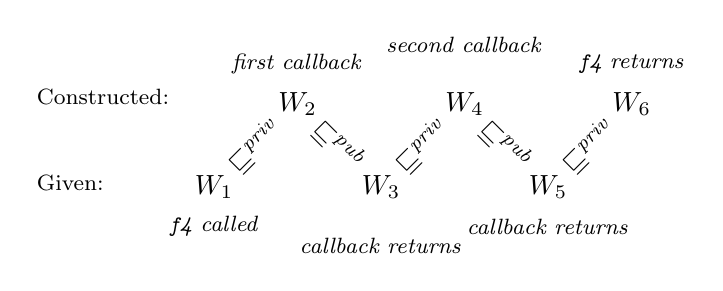
\begin{tikzpicture}[main node/.style={}, node distance=1.5cm]
  \node[main node] (1) {$W_1$};
  \node[main node] (label1) [below of=1,yshift=1cm] {\footnotesize{\textit{\texttt{f4} called}}};
  \node[main node,left] (given) [left of=1,yshift=0.05cm] {\parbox{1.5cm}{\footnotesize{Given:}}};

  \node[main node] (2) [above right of=1]{$W_2$};
  \node[main node] (label2) [above of=2,yshift=-1cm] {\textit{\footnotesize{first callback}}};

  \node[main node,left] (const) [above of=given,yshift=-0.4cm] {\parbox{1.5cm}{\footnotesize{Constructed:}}};

  \node[main node] (3) [below right of=2]{$W_3$};
  \node[main node] (label3) [below of=3,yshift=0.75cm] {\footnotesize{\textit{callback returns}}};

  \node[main node] (4) [above right of=3]{$W_4$};
  \node[main node] (label4) [above of=4,yshift=-0.75cm] {\footnotesize{\textit{second callback}}};

  \node[main node] (5) [below right of=4]{$W_5$};
  \node[main node] (label5) [below of=5,yshift=1cm] {\footnotesize{\textit{callback returns}}};

  \node[main node] (6) [above right of=5]{$W_6$};
  \node[main node] (label6) [above of=6,yshift=-1cm] {\footnotesize{\textit{\texttt{f4} returns}}};
  \path(1) edge[draw=none] node [sloped, auto=false, allow upside down] {$\sqsubseteq^\priv$} (2)
       (2) edge[draw=none] node [sloped, auto=false, allow upside down] {$\sqsubseteq^\pub$} (3)
       (3) edge[draw=none] node [sloped, auto=false, allow upside down] {$\sqsubseteq^\priv$} (4)
       (4) edge[draw=none] node [sloped, auto=false, allow upside down] {$\sqsubseteq^\pub$} (5)
       (5) edge[draw=none] node [sloped, auto=false, allow upside down] {$\sqsubseteq^\priv$} (6);
\end{tikzpicture}
\caption{Illustration of the worlds in the proof of
  Lemma~\ref{lem:correctness-g1}. In the proof, the top row of worlds are
  constructed by us, while the bottom row of worlds are given. $W_6$ is constructed such
  that $W_6 \futurestr W_5$ \emph{ and } $W_6 \futurewk W_1$.}
  \label{fig:worlds-in-pf-g1}
\end{figure}
\end{comment}
\begin{comment}
\begin{itemize}
\item Ticket dispenser
\item The awkward example and variants
\item A sandboxing example?

For example, an untrusted advertisement scenario with initialization code
that registers a redraw callback. The redraw callback gets temporary
read-write access to a framebuffer.

\item Some compartmentalization result?
\end{itemize}
\end{comment}

\section{Discussion}
\label{sec:discussion}
\noindent\textbf{Calling convention}\\
\emph{Formulating control flow correctness} While we claim that our calling
convention enforces control-flow correctness, we do not prove a general theorem
that shows this, because it is not clear what such a theorem should look like.
Formulations in terms of a control-flow graph, like the one by
\cite{abadi_control-flow_2005}, do not take into account temporal properties,
like the well-bracketedness that Example~\texttt{\footnotesize{g1}} relies on.
In fact, our examples show that our logical relation imply a stronger form of
control-flow correctness than such formulations, although this is not made very
explicit. As future work, we consider looking at a more explicit and useful way
to formalize control-flow correctness. The idea would be to define a variant
of our capability machine with call and return instructions and
well-bracketed control flow built-in to the operational semantics, and then
prove that compiling such code to our machine using our calling convention is
fully abstract~\cite{abadi_protection_1998}.

\emph{Performance and the requirement for stack clearing} The additional
security measures of the calling convention described in
\sectionname~\ref{sec:stack-and-return-pointer} impose an overhead compared to a
calling convention without security guarantees. However, most of our security
measures require only a few atomic checks or register clearings on boundary
crossings between trusted code and adversary, which should produce an acceptable
performance overhead. The only exception are the requirements for stack clearing
that we have in two situations: when returning to the adversary and when
invoking an adversary callback. As we have explained, we need to clear all of
the stack that we are not using ourselves, not just the part that we have
actually used. In other words, on every boundary cross between trusted code and
adversary code, a potentially large region of memory must be cleared. We believe
this is actually a common requirement for typical usage scenarios of local
capabilities and capability machines like CHERI should consider to provide
special support for this requirement, in the form of a highly-optimized
instruction for erasing a large block of memory. Nevertheless, from a discussion
with the designers of the CHERI capability machine, we gather that it is not immediately
clear whether and how such a primitive could be implemented efficiently in the CHERI context.

\emph{Modularity} It is important that our calling convention is modular, i.e.\ 
we do not assume that our code is specially privileged w.r.t.\ the adversary, and
they can apply the same measures to protect themselves from us as we do to
protect ourselves from them. More concretely, the requirements we have on
callbacks and return pointers received from the adversary are also satisfied by
callbacks and return pointers that we pass to them. For example, our return
pointers are local capabilities because they must point to memory where we can
store the old stack pointer, but the adversary's return pointers are also
allowed to be local. Adversary callbacks on the other hand are required to
be global but the callbacks we construct ourselves are allocated on the heap and
also global. 

\emph{Arguments and local capabilities} 
%Stack and return pointer
%Local capabilities cannot be "freely used"
%Safety dictated by LR
%Need to dynamical check whether we overwrite our local stuff.
Local capabilities are a central part of the calling convention as they are used
to construct stack and return pointers. The use of local capabilities for the
calling convention unfortunately limits the extent to which local capabilities
can be used for other things. Say we are using the calling convention and
receive a local capability other than the stack and return pointer, then we need
to be careful if we want to use it because it may be an alias to the stack
pointer. That is, if we first push something to the stack and then write to the
local capability, then we may be (tricked into) overwriting our own local state.
The logical relation helps by telling us what we need to ascertain or check in
such scenarios to guarantee safety and preserve our invariants, but such checks
may be costly and it is not clear to us whether there are practical scenarios
where this might be realistic.

%Pass capability on
%Stack example
%Pass argument by reference
%Sofisticated deep safety analysis
We also need to be careful when we receive a capability from an adversary that
we want to pass on to a different (instance of the) adversary. It turns out that
the logical relation again tells us when this is safe. Namely, the logical
relation says that we can only pass on safe arguments. For instance, when we
receive a stack pointer from an adversary, then we may at some point want to
pass on part of this stack pointer to, say, a callback. In order to do so, we
need to make sure the stack pointer is safe which means that, if we have revoked
temporary invariants, the stack must not directly or indirectly allow access to
local values that we cannot guarantee safety of. When received from an
adversary, we have to consider the contents of the stack unsafe, so before we
pass it on, we have to clear it, or perform a dynamic safety analysis of the
stack contents and anything it points to. Clearing everything is not always
desirable and a dynamic safety analysis is hard to get right and potentially
expensive.

% Can local capabilities be used for other things?/Local capabilities only for stack?
%Not unheard of - other machine also have things specific for language features.
In summary, the use of local capabilities for other things than stack and return
pointers is likely only possible in very specific scenario's when using our
calling convention. While this is unfortunate, it is not unheard of that
processors have built-in constructs that are exclusively used for handling
control flow, such as, for example, the call and return instructions that exist
in some instruction sets.
% Old version of the above:
% Carefully constructing stack and return
% pointer plays a big part in the calling convention, but it is completely
% undermined if an unsafe argument, say the full stack pointer that include the
% caller's local stack frame, is passed as an argument of the call. The logical
% relation dictates when it is safe to pass an argument to an adversary, namely it
% must be a safe value. In order to illustrate what this means for local
% capabilities, consider the stack capability. When the stack capability is
% received from an adversary, then the contents of the stack is unknown and must
% thus be considered unsafe, so before the stack capability can be passed on, we
% must make sure that it only gives access to safe values. In order to meet this
% requirement, we take a conservative approcah and simply clear everything on the
% stack. Integers are always safe, so the stack capability can now safely be
% passed on. While this approach works for the stack, it may in practice be a bit
% too naive for other local capabilities received form an adversary. Say we
% receive a capability from an adversary that happens to be the first part of the
% stack. We want to pass this capability on, so we naively clear the contents it
% gives access to which in the worst case means we overwrite our local data or the
% activation record. While this is strictly speaking not unsafe (integers are
% always) safe, it is not desirable in a real system. We would in principle also
% like to be able to pass on arguments by reference, e.g a local capability for
% some array of values. In this case, it would not be satisfactory to just clear the
% entire thing. However, the capability still needs to be safe, so there would
% need to be some kind of deep dynamic check that ensures that everything the
% capability gives access to is indeed safe. In a real setting, this may again be
% undesirable.
% This also points to a more
% general problem: When can we use local capabilities we have received from an
% adversary. We at least need to do some kind of dynamic range check to make sure
% that we do not inadverdently overwrite our local stack frame.

\emph{Single stack} A single stack is a good choice for the simple capability
machine presented here, because it works well with higher-order functions. An
alternative to a single stack would be to have a separate stack per component.
The trouble with this approach is that, with multiple stacks and local stack
pointers, it is not clear how components would retrieve their stack pointer upon
invocation without compromising safety. A safe approach could be to have stack
pointers stored by a central, trusted stack management component, but it is not
clear how that could scale to large numbers of separate components. Handling
large numbers of components is a requirement if we want to use
capability machines to enforce encapsulation of, for example, every object in an
object-oriented program or every closure in a functional program.
\\\\
% \noindent \textbf{Reasoning about capability machine programs}\\
% \emph{Semantic, but not syntactic properties} The logical relation defined in
% \sectionname~\ref{sec:logical-relation} allows us to reason about capability machine
% programs. A limitation w.r.t. previous work is that the logical relation is
% tailored exclusively towards semantic properties, not syntactic ones.

% Imagine, for example, that we invoke a block of adversary code in such a way
% that it only ever receives capabilities within a specific range of memory. After
% the code returns, we may try to prove that any capabilities passed back to us in
% the registers are still confined to that range of memory. The property of
% falling in a certain address range is syntactic in the sense that it talks about
% the specific implementation of a higher-order value rather than its behavior,
% like the invariants that are required/preserved when we use it.

% Such syntactic properties are hard to prove in our system. For the example
% cited, it would be easy to conclude that the returned values are in the value
% relation (see Figure~\ref{fig:logrel}). This gives us a lot of semantic
% information, like conditions under which they are safe to use and invariants
% that will be preserved when we do, but it does not tell us much about the
% address of the capability. As a very concrete example, capabilities with
% permission $\noperm$ are always in the value relation, irrespective of their
% address. Semantically, this makes perfect sense, since they are always safe
% since they cannot be used for anything anyway. However, it also means we do not
% get syntactic information about them.

% For our purposes, this restriction is unproblematic, since we are only
% interested in proving semantic properties (e.g., an assertion will never fail).
% However, in other situations, we may be interested in proving more syntactic
% properties like the ones that are often considered in object capability
% literature: confinement, no authority amplification etc. Although such
% properties are more restrictive and less easy to use for reasoning,
% \cite{Devriese:2016ObjCap} have demonstrated how a logical relation like
% ours can be adapted to also support them, by quantifying the logical relation
% over a custom interpretation of effectful computations and the type of
% references. We expect their solution can be readily adapted to our setting,
% modulo some details (like the fact that we do not just have read-write
% capabilities, but also others).
% % \emph{No program logic} TODO: discuss this? 
% \\\\
\noindent\textbf{Logical relation}\\
\emph{Single orthogonal closure} The definitions of $\stder$ and $\stdvr$ in
Figure~\ref{fig:logrel} apply a single orthogonal closure, a new variant of an
existing pattern called biorthogonality. Biorthogonality is a pattern for
defining logical relations~\cite{krivine_classical_1994,pitts_operational_1998}
in terms of an observation relation of safe configurations (like we do). The
idea is to define safe evaluation contexts as the set of contexts that produce
safe observations when plugging safe values and define safe terms as the set of
terms that can be plugged into safe evaluation contexts to produce safe
observations. This is an alternative to more direct definitions where safe terms
are defined as terms that evaluate to safe values. An advantage of
biorthogonality is that it scales better to languages with control effects like
call/cc. Our definitions can be seen as a variant of biorthogonality, where we
take only a single orthogonal closure: we do not define safe evaluation contexts
but immediately define safe terms as those that produce safe observations when
plugged with safe values. This is natural because we model arbitrary assembly
code that does not necessarily respect a particular calling convention: return
pointers are in principle values like all others and there is no reason to treat
them specially in the logical relation.

Interestingly, \cite{Hur:2011:KLR:1926385.1926402} also use a step-indexed,
Kripke logical relation for an assembly language (for reasoning about correct
compilation from ML to assembly), but because they only model non-adversarial
code that treats return pointers according to a particular calling convention,
they can use standard biorthogonality rather than a single orthogonal closure
like us.


\emph{Public/private future worlds} A novel aspect of our logical relation is
how we model the temporary, revokable nature of local capabilities using public/private
future worlds. The main insight is that this special nature generalizes that of the syntactically-enforced
unstorable status of evaluation contexts in lambda calculi without control
effects (of which well-bracketed control flow is a consequence). To reason about
code that relies on this (particularly, the original awkward example),
\cite{Dreyer:jfp12} (DNB) formally capture the special status of evaluation
contexts using Kripke worlds with public and private future world relations.
Essentially, they allow relatedness of evaluation contexts to be monotone with
respect to a weaker future world relation (public) than relatedness of values,
formalizing the idea that it is safe to make temporary internal state
modifications (private world transitions, which invalidate the continuation,
but not other values) while an expression is performing internal steps, as long
as the code returns to a stable state (i.e. transitions to a public future world
of the original) before returning. We
generalize this idea to reason about local capabilities: validity of local
capabilities is allowed to be monotone with respect to a weaker future-world
relation than other values, which we can exploit to distinguish between state
changes that are always safe (public future worlds) and changes that are only
valid if we clear all local capabilities (private future worlds). Our future
world relations are similar to DNB's (for example, our proof of
the awkward example uses exactly the same state transition system),
but they turn up in an entirely different place in the logical relation: rather
than using public future worlds for the special syntactic category of evaluation
contexts, they are used in the value relation depending on the
locality of the capability at hand. Additionally, our worlds are a bit more
complex because, to allow local memory capabilities and write-local
capabilities, they can contain (revokable) temporary regions that are only
monotonous w.r.t. public future worlds, while DNB's worlds are entirely
permanent.

\emph{Local capabilities in high-level languages} We point out that
local capabilities are quite similar to a feature proposed for the high-level
language Scala: \cite{osvald_gentrification_2016}'s second-class or local
values. They are a kind of values that can be provided to other code for
immediate use without allowing them to be stored in a closure or reference for
later use. We believe reasoning about such values will require techniques similar 
to what we provide for local capabilities.

\section{Related work}
\label{sec:related-work}

Finally, we summarize how our work relates to previous work. We do not
repeat the work we discussed in \sectionname~\ref{sec:discussion}.

Capability machines originate with \cite{Dennis:1966:PSM:365230.365252} and we refer to
\cite{Levy1984capability} and \cite{Watson2015Cheri} for an overview
of previous work. The capability machine formalized in
\sectionname~\ref{sec:capab-mach-with} is a simple but representative
model, modeled mainly after the
M-Machine~\cite{Carter:1994:HSF:195473.195579} (the enter pointers
resemble the M-Machine's) and
CHERI~\cite{Watson2015Cheri,Woodruff:2014:CCM:2665671.2665740} (the
memory and local capabilities resemble CHERI's). The latter is a
recent and relatively mature capability machine, which combines
capabilities with a virtual memory approach, in the interest of
backwards compatibility and gradual adoption. As discussed, our local
capabilities can cross module boundaries, 
contrary to what is enforced by CHERI's default CCall implementation.

Plenty of other papers\lau{If there are plenty, then I guess we should cite more
  than one?} enforce well-bracketed control flow at a low level, but most are
restricted to preventing particular types of attacks and enforce only partial
correctness of control flow. This includes particularly the line of work on
\emph{control-flow integrity}~\cite{abadi_control-flow_2005}. Those use a quite
different attacker model than us: they assume an attacker that is not able to
execute code, but can overwrite arbitrary data at any time during execution (to
model buffer overflows). By checking the address of every indirect jump and
using memory access control to prevent overwriting code, this work enforces what
they call control-flow integrity, formalized as the property that every jump
will follow a legal path in the control-flow graph. As discussed in
\sectionname~\ref{sec:discussion}, such a property ignores temporal properties and
seems hard to use for reasoning.

More closely related to our work are papers that use a trusted stack manager and
some form of memory isolation to enforce control-flow correctness as part of a
secure compilation
result \cite{patrignani_modular_2016-1,juglaret_beyond_2016-1}. Our work
differs from theirs in that we use a different form of low-level security
primitive (a capability machine with local capabilities rather than a machine
with a primitive notion of compartments) and we do not use a trusted stack
manager, but a decentralized calling convention based on local
capabilities. Also, both prove a secure compilation result from a high-level
language, which clearly implies a general form of control-flow correctness,
while we define a logical relation that can be used to reason about
specific programs that rely on well-bracketed control flow.

Our logical relation is a unary, step-indexed Kripke logical relation with
recursive worlds
\cite{pitts_operational_1998,Appel:2001:IMR:504709.504712,Ahmed2004semantics,Birkedal:2011:SKM:1926385.1926401},
closely related to the one used by \cite{Devriese:2016ObjCap} to formulate
capability safety in a high-level JavaScript-like lambda calculus. Our
Fundamental Theorem is similar to theirs and expresses capability safety of the
capability machine. Because we are not interested in externally observable
side-effects (like console output or memory access traces), we do not require
their notion of effect parametricity. Our logical relation uses several ideas
from previous work, like Kripke worlds with regions containing state transition
systems \cite{Ahmed:popl09}, public/private future worlds \cite{Dreyer:jfp12}
(see \sectionname~\ref{sec:discussion} for a discussion), and biorthogonality
\cite{pitts_operational_1998,benton_biorthogonality_2009-1,Hur:2011:KLR:1926385.1926402}.

Swasey et. al.~\cite{swasey:2017} have recently developed a \emph{logic}, OCPL, for verification
of object capability patterns. The logic is based on
Iris~\cite{iris,iris2,iris3}, a state of the art higher-order concurrent
separation logic and is formalized in Coq, building on the Iris Proof Mode for
Coq~\cite{ipm}. OCPL gives a more abstract and modular way of proving
capability safety for a lambda-calculus (with concurrency) compared to the
earlier work by \cite{Devriese:2016ObjCap}.
%domi: rest of the paragraph could be cut?
% In the future we would also like to
% investigate a new program logic for reasoning about capability safety for our
% capability machine model. We think Iris would also be a natural starting point
% for such an endeavour, since Iris is really a framework, which can be
% instantiated to different programming languages. OCPL was able to leverage
% existing Iris specifications for the high-level language; for our capability
% machine model, however, it would be necessary to devise new kinds of
% specifications for our low-level programs with unstructured control-flow. It is
% likely that we could get inspiration from earlier work on logics for assembly
% programming languages, such as XCAP~\cite{xcap}.

El-Korashy also defined a formal model of a capability machine, namely CHERI,
and uses it to prove a compartmentalization
result~\cite{akram_el-korashy_formal_2016} (not implying control-flow
correctness). He also adapts control-flow integrity (see above) to the machine
and shows soundness, seemingly without relying on capabilities.


%% Acknowledgments
% \begin{acks}                            %% acks environment is optional
%                                         %% contents suppressed with 'anonymous'
%   %% Commands \grantsponsor{<sponsorID>}{<name>}{<url>} and
%   %% \grantnum[<url>]{<sponsorID>}{<number>} should be used to
%   %% acknowledge financial support and will be used by metadata
%   %% extraction tools.
%   This material is based upon work supported by the
%   \grantsponsor{GS100000001}{National Science
%     Foundation}{http://dx.doi.org/10.13039/100000001} under Grant
%   No.~\grantnum{GS100000001}{nnnnnnn} and Grant
%   No.~\grantnum{GS100000001}{mmmmmmm}.  Any opinions, findings, and
%   conclusions or recommendations expressed in this material are those
%   of the author and do not necessarily reflect the views of the
%   National Science Foundation.
% \end{acks}


%% Bibliography
\bibliography{references}


%% Appendix
% \appendix
% \section{Appendix}

% Text of appendix \ldots

\end{document}
